\documentclass[12pt]{report}
\usepackage[greek]{babel}
\usepackage{fontspec}
\usepackage{graphicx}
\usepackage{booktabs}
%!TEX TS-program = xelatex
%!TEX encoding = UTF-8 Unicode
\usepackage{xltxtra}
\usepackage{titlesec}
\setmainfont{Times New Roman}
\usepackage{subcaption}
\usepackage[export]{adjustbox}
\usepackage{wrapfig}
\usepackage[a4paper, 
    top=3cm, 
    bottom=2.54cm, 
    left=2.54cm, 
    right=2.54cm,
    headheight=28pt,  % Critical for header space
    headsep=1.2cm,
    includehead,      % Include header in page area
    includefoot]{geometry}
\usepackage{hyperref}
\usepackage{makecell}
\usepackage{float}
\usepackage{chngcntr}
\usepackage{caption}
\usepackage[justification=centering]{caption}
\usepackage[noabbrev]{cleveref}

\usepackage[font={smaller,it}]{caption}
\usepackage[backend=biber, style=apa, sorting=ynt]{biblatex}
\usepackage{setspace}
\usepackage{tablefootnote}
\usepackage{csquotes}
\usepackage{fancyhdr}
\usepackage{etoolbox}
\usepackage{tocloft}
\usepackage{listings}
\usepackage{cleveref}
\usepackage{xcolor}
\addbibresource{references.bib}
\usepackage{nomencl}
\usepackage[table]{xcolor}
\usepackage{multirow}
\captionsetup{tablename=Πίνακας}
\renewcommand\theadfont{\bfseries}
\renewcommand{\arraystretch}{1.5}

% \pagestyle{fancy}
% \fancyhf{} % Clear all headers/footers
% \addto\captionsgreek{%
%   \crefname{lstlisting}{κώδικας}{κώδικες}%
%   \Crefname{lstlisting}{Κώδικας}{Κώδικες}%
%   \crefname{appendix}{παράρτημα}{παραρτήματα}%
%   \Crefname{appendix}{Παράρτημα}{Παραρτήματα}%
% }

\captionsetup[figure]{
  labelformat=simple,
  labelsep=space,
  name=Εικόνα,
  format=plain
}
\counterwithin{figure}{chapter}

\captionsetup[table]{
  labelformat=simple,
  labelsep=space,
  name=Πίνακας,
  format=plain
}
\counterwithin{table}{chapter}

\renewcommand{\thesubfigure}{\roman{subfigure}}
\renewcommand{\thesubtable}{\roman{subtable}}

\titleformat{\chapter}[display]
    {\fontsize{16pt}{18pt}\selectfont\bfseries\raggedright}
    {\appendixname\ \thechapter}
    {0pt}
    {}
\titlespacing*{\chapter}{0pt}{0pt}{18pt}

\lstset{
    basicstyle=\fontsize{9}{11}\selectfont\ttfamily, % Courier New equivalent
    breaklines=true,
    frame=single,
    numbers=left,
    numberstyle=\tiny,
    stepnumber=1,
    tabsize=4,
    backgroundcolor=\color{gray!5},
    keywordstyle=\color{blue},
    commentstyle=\color{green!50!black},
    stringstyle=\color{red},
    showstringspaces=false
}

\fancypagestyle{mainstyle}{
    \fancyhf{}
    \fancyhead[L]{\hspace{2em}
\includegraphics[height=1.21cm,width=3.24cm]{university1-logo.png}}
    \fancyhead[C]{\raisebox{1ex}{%
        \parbox{\dimexpr\textwidth-7.5cm-4em\relax}{%
            \itshape\footnotesize%
            Κωνσταντίνος Περπερίδης\\%
            Ανάλυση δεδομένων γονιδιακής έκφρασης\\%
            και χαρτογράφηση λειτουργικών δικτύων\\%
            στη νόσο του Πάρκινσον%
        }}}
    \fancyhead[R]{
\includegraphics[height=1.21cm,width=4cm]{university2-logo.png}\hspace{2em}}
    \fancyfoot[C]{\thepage}
    \renewcommand{\headrulewidth}{0pt}
    % Remove the headsep from here since we set it in geometry
}


\fancypagestyle{plain}{
    \fancyhf{}
    \fancyfoot[C]{\thepage}
    \renewcommand{\headrulewidth}{0pt}
}

\makeatletter

\let\oldchapter\chapter
\renewcommand{\chapter}{\@ifstar{\starchapter}{\nostarchapter}}
\newcommand{\starchapter}[1]{\oldchapter*{#1}\thispagestyle{mainstyle}}
\newcommand{\nostarchapter}[1]{\oldchapter{#1}\thispagestyle{mainstyle}}
\makeatother

\makenomenclature
\renewcommand{\nomname}{Συντομογραφίες και Ακρωνύμια} % Custom title
\renewcommand{\nomlabelwidth}{2.5cm} % Adjust as needed

% Formatting to match your document
\renewcommand{\nompreamble}{\vspace{6pt}} % Space before list
\setlength{\nomitemsep}{6pt} 

% Reduce spacing in TOC
\setlength{\cftbeforechapskip}{6pt} % Space before chapter entries (was ~10pt)
\setlength{\cftbeforesecskip}{3pt} % Space before section entries
\setlength{\cftbeforesubsecskip}{3pt} % Space before subsection entries

% Add dot leaders for chapters (normally missing in report class)
\renewcommand{\cftchapleader}{\cftdotfill{\cftdotsep}} % Dot leaders for chapters
\renewcommand{\cftsecleader}{\cftdotfill{\cftdotsep}} % Ensures section leaders
\renewcommand{\cftsubsecleader}{\cftdotfill{\cftdotsep}} % Subsection leaders

% Font settings for TOC entries
\renewcommand{\cftchapfont}{\normalfont} % Chapter font
\renewcommand{\cftchappagefont}{\normalfont} % Chapter page number font

\onehalfspacing % 1.5 line spacing

% Header settings
\newlength{\logoheight}
\setlength{\logoheight}{1.21cm}
\newlength{\logowidth}
\setlength{\logowidth}{3.24cm}
\newlength{\headertextwidth}
\setlength{\headertextwidth}{\dimexpr\textwidth-2\logowidth-2em\relax}

\newcommand{\frontmatter}{
    \cleardoublepage
    \pagenumbering{roman}
    \pagestyle{plain} % Simple page numbers only
    \setcounter{page}{1} % Explicit reset
}

% Chapter formatting
\titleformat{\chapter}[display]
    {\fontsize{16pt}{18pt}\selectfont\bfseries\raggedright}
    {\thechapter}
    {0pt}
    {}
\titlespacing*{\chapter}{0pt}{0pt}{18pt}

% Section formatting
\titleformat{\section}
    {\fontsize{14pt}{12pt}\selectfont\bfseries\raggedright}
    {\thesection}
    {1em}
    {}
\titlespacing*{\section}{0pt}{12pt}{12pt}

% Subsection formatting
\titleformat{\subsection}
    {\fontsize{12pt}{6pt}\selectfont\bfseries\raggedright}
    {\thesubsection}
    {1em}
    {}
\titlespacing*{\subsection}{0pt}{0pt}{6pt}

% Subsubsection formatting
\titleformat{\subsubsection}
    {\fontsize{12pt}{6pt}\selectfont\bfseries\itshape\raggedright}
    {}
    {0pt}
    {}
\titlespacing*{\subsubsection}{0pt}{0pt}{6pt}

% Paragraph settings
\setlength{\parindent}{0pt}
\setlength{\parskip}{6pt}

% Caption settings
\captionsetup{
    font=footnotesize,
    labelfont=bf,
    justification=centering,
    singlelinecheck=off,
    skip=6pt,
    belowskip=12pt
}
\DeclareCaptionLabelFormat{chapter}{\thechapter.#1}
% \captionsetup[figure]{labelformat=chapter}
% \captionsetup[table]{labelformat=chapter}

% Prevent figure/table captions from breaking across pages
% \pretocmd{\figure}{\begin{minipage}{\linewidth}}{}{}
% \apptocmd{\endfigure}{\end{minipage}}{}{}
% \pretocmd{\table}{\begin{minipage}{\linewidth}}{}{}
% \apptocmd{\endtable}{\end{minipage}}{}{}

% Footnote settings
\renewcommand{\footnotesize}{\fontsize{10pt}{1}\selectfont}
\let\oldfootnote\footnote
\renewcommand{\footnote}[1]{\oldfootnote{\onehalfspacing #1}}


% \title{\fontsize{16pt}{18pt}\selectfont\bfseries Ανάλυση δεδομένων γονιδιακής έκφρασης και χαρτογράφηση λειτουργικών δικτύων στη νόσο του Πάρκινσον}
% \author{Κωνσταντίνος Περπερίδης}
% \date{\today}
% \maketitle

\makeatletter
\renewcommand{\@makechapterhead}[1]{%
  \vspace*{0pt}%
  {\parindent \z@ \raggedright \normalfont
    \fontsize{16pt}{18pt}\selectfont\bfseries
    \mbox{\thechapter.\ #1}\par
    \nobreak
    \vskip 18pt
  }}
\makeatother

\makeatletter
\newcommand{\addtotoc}[1]{
    \cleardoublepage
    \phantomsection
    \addcontentsline{toc}{chapter}{#1}
}
\renewcommand{\maketitle}{
    \begin{titlepage}
        % \null\vfill
        \noindent
        \begin{minipage}[t]{0.6\textwidth}
            \centering
            
\includegraphics[height=2.4cm,width=6cm]{university1-logo.png}\\
            \fontsize{12pt}{14pt}\selectfont
            Σχολή Θετικών Επιστημών και Τεχνολογίας
        \end{minipage}
        \hfill
        \begin{minipage}[t]{0.4\textwidth}
            \centering
            
\includegraphics[height=1.8cm,width=6.5cm]{university2-logo.png}\\
            \fontsize{12pt}{14pt}\selectfont
            Τμήμα Πληροφορικής
        \end{minipage}
        \vspace*{2cm}
        \begin{center}
            \fontsize{16pt}{14pt}\selectfont
            Διαπανεπιστημιακό Μεταπτυχιακό Πρόγραμμα Σπουδών\\[14pt]
            Βιοπληροφορική και Νευροπληροφορική\\[48pt]
            Μεταπτυχιακή Διπλωματική Εργασία\\[24pt]
    
            {\fontsize{16pt}{18pt}\selectfont\bfseries \@title\\[18pt]}
            {\large \@author\\[12pt]}\\[24pt]
            \fontsize{12pt}{14pt}\selectfont
            Επιβλέπων καθηγητής: Μάριος Κροκίδης\\
            \vspace{5cm}
            \fontsize{14pt}{16pt}\selectfont
            Κιλκίς, {\large \@date}
        \end{center}
        % \vfill\null
    \end{titlepage}
}
\makeatother

% Document body
\begin{document}
\frontmatter

\title{Ανάλυση δεδομένων γονιδιακής έκφρασης και χαρτογράφηση λειτουργικών δικτύων στη νόσο του Πάρκινσον}
\author{Κωνσταντίνος Περπερίδης}
\date{\today}
\maketitle
\thispagestyle{empty} 
\cleardoublepage
\thispagestyle{empty} 
\vspace*{\fill} % Push content to vertical center
\begin{center}
\fontsize{10pt}{12pt}\selectfont
\textcopyright
Η παρούσα εργασία αποτελεί πνευματική ιδιοκτησία του/της φοιτητή/φοιτήτριας («συγγραφέας/δημιουργός»)
που την εκπόνησε. Στο πλαίσιο της πολιτικής ανοικτής πρόσβασης ο συγγραφέας/δημιουργός εκχωρεί στο
ΕΑΠ, μη αποκλειστική άδεια χρήσης του δικαιώματος αναπαραγωγής, προσαρμογής, δημόσιου δανεισμού,
παρουσίασης στο κοινό και ψηφιακής διάχυσής τους διεθνώς, σε ηλεκτρονική μορφή και σε οποιοδήποτε
μέσο, για διδακτικούς και ερευνητικούς σκοπούς, άνευ ανταλλάγματος και για όλο το χρόνο διάρκειας των
δικαιωμάτων πνευματικής ιδιοκτησίας. Η ανοικτή πρόσβαση στο πλήρες κείμενο για μελέτη και ανάγνωση
δεν σημαίνει καθ’ οιονδήποτε τρόπο παραχώρηση δικαιωμάτων διανοητικής ιδιοκτησίας του
συγγραφέα/δημιουργού ούτε επιτρέπει την αναπαραγωγή, αναδημοσίευση, αντιγραφή, αποθήκευση, πώληση,
εμπορική χρήση, μετάδοση, διανομή, έκδοση, εκτέλεση, «μεταφόρτωση» (downloading), «ανάρτηση»
(uploading), μετάφραση, τροποποίηση με οποιονδήποτε τρόπο, τμηματικά ή περιληπτικά της εργασίας, χωρίς
τη ρητή προηγούμενη έγγραφη συναίνεση του συγγραφέα/δημιουργού. Ο συγγραφέας/δημιουργός διατηρεί
το σύνολο των ηθικών και περιουσιακών του δικαιωμάτων.
\end{center}
\vspace*{\fill} % Ensure it stays at bottom
\clearpage


\clearpage
\thispagestyle{empty} % No header/footer
\begin{center}
    
    \begin{minipage}[t]{0.45\textwidth}
        \centering
        
\includegraphics[height=2.4cm,width=6cm]{university1-logo.png}\\
    \end{minipage}
    \hfill
    \begin{minipage}[t]{0.45\textwidth}
        \centering
        
\includegraphics[height=1.8cm,width=6.5cm]{university2-logo.png}\\
    \end{minipage}
    \vspace*{2cm}
    
    \fontsize{18pt}{22pt}\selectfont\
        Ανάλυση δεδομένων γονιδιακής έκφρασης και χαρτογράφηση λειτουργικών δικτύων στη νόσο του Πάρκινσον\\
    \vspace*{2.5cm}
    \large Κωνσταντίνος Περπερίδης\\
    \vspace*{2.5cm}
    \begin{center}
    \fontsize{12pt}{14pt}\selectfont
    Επιτροπή Επίβλεψης Διπλωματικής Εργασίας\\[16pt]
    \begin{minipage}[t]{0.45\textwidth}
        \centering
        \fontsize{12pt}{14pt}\selectfont
        \textbf{Επιβλέπων Καθηγητή}\\
        Μάριος Κροκίδης\\
        Επίκουρος Καθηγητής - Ιόνιο Πανεπιστήμιο
    \end{minipage}
    \hfill % Maximizes horizontal space between minipages
    \begin{minipage}[t]{0.45\textwidth}
        \centering
        \fontsize{12pt}{14pt}\selectfont
        \textbf{Συν-Επιβλέπων Καθηγητής}\\
        Θεμιστοκλής Έξαρχος\\
        Αναπληρωτής Καθηγητής - Ιόνιο Πανεπιστήμιο
    \end{minipage}
    \end{center}
    \vspace*{2.5cm}
    \fontsize{14pt}{16pt}\selectfont
    Κιλκίς, {\large \today}
    
    \vfill
\end{center}
\clearpage

\cleardoublepage
\pagestyle{mainstyle}

\chapter*{Περίληψη}
\addcontentsline{toc}{chapter}{Περίληψη}
    \par
        H εργασία αυτή διαπραγματεύεται την ανάλυση μεταγραφικών δεδομένων αλληλούχισης RNA από δείγματα ολικού αίματος, καθώς και την χαρτογράφηση πιθανών λειτουργικών δικτύων στη νόσο του Πάρκινσον. Σκοπό αποτελεί η εφαρμογή κατάλληλων βιοπληροφοριακών εργαλείων προκειμένου να εντοπιστούν διαφορές στη γονιδιακή έκφραση μεταξύ συγκεκριμένων δεδομένων της νόσου και παράλληλα να αναζητηθούν γονίδια-στόχοι που εμπλέκονται στην παθοφυσιολογία.
    \par
        Η νόσος του Πάρκινσον χαρακτηρίζεται από έντονη κινητική δυσχέρεια με χαρακτηριστικό τρόμο στα άκρα και οφείλεται στην απώλεια ντοπαμινεργικών νευρώνων στην μέλαινα ουσία του εγκεφάλου. Η απώλεια λειτουργικών νευρώνων οδηγεί στην μείωση έκλυσης του νευροδιαβιβαστή της Ντοπαμίνης και οφείλεται στην συσσώρευση της πρωτεΐνης α-Συνουκλεϊνης και τη διαμόρφοση των λεγόμενων σωμάτιων Lewy εντός του κυττοπλάσματος των ντοπαμινεργικών νευρώνων (\emph{\cite{Balestrino2020ParkinsonDisease}}).
    \par
        Τα δείγματα προέρχονται από μια εκτεταμένη μελέτη, την Parkinson Progression Markers Initiative \emph{(PPMI\footnote{https://www.ppmi-info.org/})} τα οποία διανέμονται διαδικτυακά κατόπιν εγγραφής στις σελίδας του Imaging and Data Archive \emph{(IDA\footnote{https://ida.loni.usc.edu/})}. Πρόκειται για μια πολυδιάστατη μελέτη, καθώς πέραν των δεδομένων αλληλούχισης μεταγραφώματος διανέμονται μεταξύ άλλων και δεδομένα πρωτεομικής, μεθυλίωσης, κλινικών μελετών και απεικονιστικών εξετάσεων από ομάδες νοσούντων, ελέγχου αλλά και ατόμων με πιθανή γενετική προδιάθεση, ως φορείς γενετικών μεταλλάξεων σε γνωστά γονίδια τα οποία εμπλέκονται στην παθοφυσιολογία της νόσου.
    \par
        Καθώς τα διαγνωστικά πρωτόκολλα στηρίζονται κατά βάση σε κλινική αξιολόγηση των κινητικών συμπτωμάτων από ειδικούς νευρολόγους. Έχουν καθιερωθεί πρωτόκολλα αξιολόγησης κλινικών συμπτωμάτων, τα οποία στηρίζουν τη διαφορική διάγνωση (\emph{\cite{Koller2018TableGuidelines}}), τα συμπτώματα που παρουσιάζουν κινητική παθολογία είναι πιθανόν να αλληλεπικαλύπτονται με άλλες παθήσεις του νευρικού συστήματος (\emph{\cite{Tolosa2021ChallengesDisease}}). 
    \par
        Μια έγκαιρη διάγνωση η οποία στηρίζεται σε βιοδείκτες, όπως ενδείξεις εγκεφαλογραφημάτων, απεικονιστικών εξετάσεων όπως αυτής της μαγνητικής τομογραφίας εγκεφάλου αλλά και βιολογικού υλικού όπως εγκεφαλονωτιαίου υγρού αλλά και προϊόντα αίματος δεν έχουν καθιερωθεί καθώς ποικίλες έρευνες διαπραγματεύονται την ανεύρεση βιοδεικτών από διάφορες πηγές του οργανισμού (\emph{\cite{Miller2015BiomarkersFuture}}) (\emph{\cite{Maitin2022SurveyReview}}).
    \par
        Στην παρούσα εργασία χρησιμοποιούνται δείγματα ολικού αίματος ως μια προσιτή και πλούσια πηγή βιολογικής πληροφορίας. Ταυτόχρονα η αφθονία μεταγραφικής πληροφορίας που εμπεριέχεται στο αίμα, καθιστά μια εξαιρετική πρόκληση στην εύρεση και διαφοροποίηση σημαντικής πληροφορίας ως προς την αναγνώριση πιθανών βιοδεικτών και λειτουργικών δικτύων που θα μπορούσαν να επιτρέψουν τον συσχετισμό με τη νόσο του Πάρκινσον.
    \par
        Τα εργαλεία της βιοπληροφορικής που χρησιμοποιήθηκαν σε αυτή τη διπλωματική εργασία είναι μέθοδοι στατιστικής ανάλυσης, όπως η διαφορική ανάλυση γονιδιακής έκφρασης, η ανάλυση εμπλουτισμού και η μηχανική μάθηση, για την ανεύρεση χαρακτηριστικών που καθιστούν πιθανή την αναγνώριση της νόσου αλλά και την διασταύρωση των αποτελεσμάτων με πληροφορίες από βάσεις δεδομένων σχολιασμού.
        
    \cleardoublepage

    \chapter*{Abstract}
    \addcontentsline{toc}{chapter}{Abstract}
        \selectlanguage{english}
            \par
                This thesis handles the analysis of transcriptome data from RNA sequencing on whole-blood samples and the mapping of functional gene networks in Parkinson's disease. It aims at the application of suitable bioinformatics toolsets in order to recognise differences in gene expressions between particular data of the disease and in parallel to search for target genes with possible involvement in the pathophysiology.
            \par
                Parkinson's disease on the surface is defined by intense movement distress with a characteristic tremor on the limbs which is assumed to be due to the loss of dopaminergic neurons in the substantia nigra of the brain. The loss of functional neurons leads to progressive reduction of the neurotransmitter Dopamine and effectively happens because of accumulation of α-Synuclein to Lewy bodies in the inside of the dopaminergic cells (\emph{\cite{Balestrino2020ParkinsonDisease}}).
            \par
                The samples used in the this thesis originate from a large-scale study, the Parkinson Progression Markers Initiative (\emph{PPMI}) which are made available to download on the internet after registration on the pages of the Imaging and Data Archive (\emph{IDA}). It is indeed a multi-dimensional study since there are results from several examinations available apart from genetic data, such as Proteomics results, Methylation profiles, Clinical studies and Imaging results from case and control cohorts and dditionally from individuals with a possible genetic predisposition as carriers of genetic mutations in genes that are known to be involved in the pathophysiology of the disease.
            \par
                Since the diagnostic protocols are based on clinical assessment of the symptoms from neurologists and standards that guide the diagnosis (\emph{\cite{Koller2018TableGuidelines}}), symptoms still may overlap with other disease of the nervous system that also have a severe impact on the locomotor system (\emph{\cite{Tolosa2021ChallengesDisease}}).
            \par
                An early diagnosis that relies on biomarkers like indications from EEG's or MRI's and also biological samples like cerebrospinal fluid and ideally non-invasive samples like blood products, haven't been established by now and several research attempts focus on biomarker discovery from different sources of the organism (\emph{\cite{Miller2015BiomarkersFuture}}) (\emph{\cite{Maitin2022SurveyReview}}).
            \newpage
            \par
                The present thesis uses whole-blood samples as a non-invasive and affordable source of information. At the same time, the abundance of transcriptomic information included in the blood bears an extraordinary challenge for the search and recognition of potential biomarkers and functional networks that could allow a correlation with Parkinson's disease.
            \par
                The bioinformatics toolset as employed in this thesis contains methods from the field of biostatistical analysis, like differential gene expression analysis or gene-set enrichment analysis and machine learning for finding potential features that could aid as diagnostical support and to validate the information against enrichment and annotation resources.
    
    \selectlanguage{greek}
    \cleardoublepage
    \tableofcontents
    \thispagestyle{mainstyle}
    \addtotoc{\contentsname}
    \cleardoublepage

    \addcontentsline{toc}{chapter}{\listfigurename}
    \listoffigures
    \thispagestyle{mainstyle}

    \cleardoublepage
    \addcontentsline{toc}{chapter}{\listtablename}
    \listoftables
    \thispagestyle{mainstyle}

    \cleardoublepage
    \printnomenclature[2.5cm] % The number sets indent
    \thispagestyle{mainstyle}
    \addcontentsline{toc}{chapter}{\nomname}
    
    % Main matter
    \cleardoublepage
    \pagestyle{mainstyle}
    \pagenumbering{arabic}
    
    \chapter{Εισαγωγή}
    \par
        Χρησιμοποιήθηκαν δεδομένα RNA από το Project 133 IR3 με τελευταία έκδοση την 4η Φεβρουαρίου 2021, σύμφωνα με τη σελίδα του PPMI\nomenclature{PPMI}{Parkinson's Progression Markers Initiative}. Το σύνολο των δειγμάτων καθώς και αρχείο CSV το οποίο περιλαμβάνει μέτα-πληροφορίες αναφορικά με τα δείγματα διενεργήθηκε μέσω Download μετά από εγγραφή στις σελίδες του παρόχου δεδομένων της μελέτης του PPMI, IDA\nomenclature{IDA}{Imaging and Data Archive}. Το συμπιεσμένο αρχείο περιλαμβάνει μεμονωμένα αρχεία για κάθε δείγμα. Υπάρχουν αρχεία με τιμές έκφρασης με κανονικοποίηση TPM\nomenclature{TPM}{Transcripts per Million} (\emph{\cite{Zhao2021TPMRepository}}) και με μετατροπή σε μορφή feature counts (\emph{\cite{Liao2014FeatureCounts:Features}}). Η ανάκτηση σε FASTQ \nomenclature{FASTQ}{Επέκταση του τύπου FASTA - Τύπος αρχείου βασισμένο σε κείμενο για την καταγραφή βιολογικών αλληλουχιών} δεν είναι δυνατή διαδικτυακά, παρά μόνο με αποστολή σκληρού δίσκου μετά από ειδική αίτηση από την έδρα του IDA στις ΗΠΑ. Πρόκειται για όγκο δεδομένων μεγέθους 184 TB\nomenclature{TB}{Tera Byte} σύμφωνα με το εγχειρίδιο \footnote{\url{https://www.ppmi-info.org/sites/default/files/docs/PPMI\%20Data\%20User\%20Guide.pdf}}.
    \par
        Στην παρούσα εργασία έγινε χρήση των feature counts μιας και η κανονικοποίηση σε TPM θα περιόριζε την καταλληλότητα των δεδομένων ως προς την ανάλυση, ειδικά σε μεθόδους όπως την ανάλυση διαφορικής έκφρασης. Αυτό οφείλεται στο γεγονός ότι η συγκεκριμένη κανονικοποίηση γενικά λειτουργεί σε επίπεδο δείγματος, καθιστώντας τα δείγματα ακατάλληλα για μια μεταξύ τους σύγκριση. Ιδανικά, τα πακέτα λογισμικού ανάλυσης γονιδιακής έκφρασης όπως DESeq (\emph{το οποίο χρησιμοποιήθηκε και σε αυτή την εργασία}) απαιτούν τα δεδομένα σε RAW, δηλαδή ακατέργαστη μορφή, χωρίς κάποια κανονικοποίηση. Δεδομένου των προϋποθέσεων για μια ανάκτηση των αντίστοιχων πληροφοριών, όπως αναφέρθηκε και παραπάνω, η μορφή feature counts φάνηκε ως η πιο κατάλληλη καθώς είναι ότι πιο κοντινό σε ακατέργαστα δεδομένα μεταγραφικής πληροφορίας.
        
    \section{Συγκρότηση και Συγχώνευση Δεδομένων}
        \par
            Τα δεδομένα της μελέτης του PPMI περιέχουν ξεχωριστά αρχεία ανά δείγμα. Για την ανάλυση είναι χρήσιμη η διάθεση ενός μοναδικού συνόλου με όλα τα δείγματα, τις τιμές έκφρασης ανά δείγμα αλλά και μέτα-πληροφορίες όπως σε ποια ομάδα, ελέγχου ή νοσούντων, ανήκει ένα δείγμα, το φύλο, η ηλικία κα. για την συγκρότηση ενός τέτοιου συνόλου συγγράφηκε το σενάριο στον κώδικα~\ref{lst:readdatapy} και το σενάριο στον κώδικα~\ref{lst:preparedatapy}. Στο πρώτο συλλέγονται τα αρχεία-δείγματα και καταγράφονται σε ένα CSV\nomenclature{CSV}{Comma Separated Values} αρχείο, ενώ στο 2ο γίνεται ανάγνωση αυτού του αρχείου, επικόλληση των μέτα-δεδομένων ανά δείγμα και εκκαθάριση του συνόλου εφαρμόζοντας φίλτρο σε στήλη η οποία ορίζει αν ένα δείγμα πληροί τα ποιοτικά κριτήρια του πειράματος ή όχι. Σαφώς στο σενάριο γίνεται εκκαθάριση όσων δειγμάτων δεν φέρουν την τιμή "pass" στην αντίστοιχη στήλη.
        \par
            Για την καλύτερη διαχείριση, σε οποιοδήποτε αναλυτικό σκέλος της εργασίας, θεωρήθηκε σκόπιμη η συγκρότηση των δεδομένων σε αντικείμενο AnnData καθώς και η αποθήκευση σε αρχείο τύπου h5ad. Ακολουθεί μια ιεραρχική δομή όπου παρέχεται εύκολη πρόσβαση σε παρατηρήσεις (\emph{obs}) και σε μεταβλητές (\emph{var}) αλλά και σε άλλες συλλογές πληροφορίας, όπως κανονικοποιημένες τιμές έκφρασης και πίνακες αντιστοίχησης με σύμβολα γονιδίων. Επιπλέων, οι μεμονομένες ηλικίες ανά άτομο συγκροτήθηκαν στις ηλικιακές ομάδες 30-50, 50-70, 70-80 και >80 (\emph{κώδικας~\ref{lst:dataconsolidationpy}}).
            \begin{figure}[h]
                \centering
                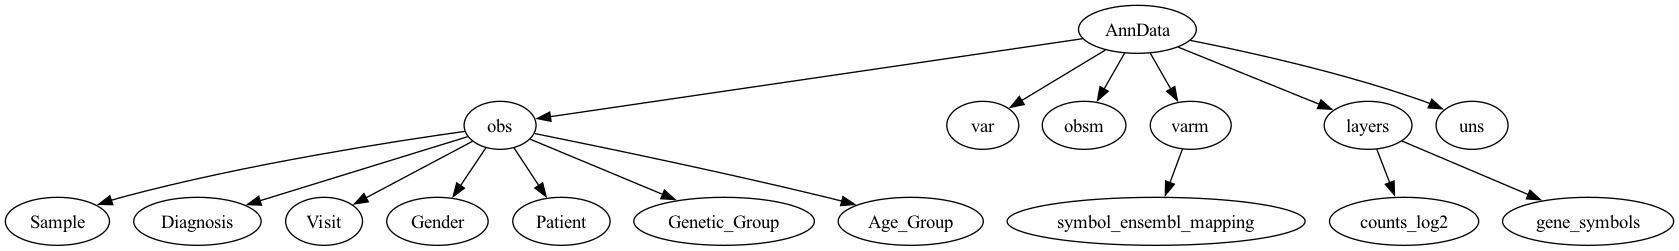
\includegraphics[width=0.8\textwidth]{anndata_structure.png}
                \caption{Δομή του AnnData αντικειμένου της εργασίας}
                \label{fig:figure-1}
            \end{figure}
    \section{Μέθοδοι}
        \par
            Το σύνολο των δεδομένων που επιλέχθηκε σε αυτή την εργασία περιέχει μερικές αξιοσημείωτες προκλήσεις για την ανάλυση. Αφενός, αυτές προκύπτουν από τη φύση των δειγμάτων αίματος, όπου η ποικιλία μεταγραφικού προϊόντος είναι πιθανόν να εμπεριέχει και βιολογικό θόρυβο, ο οποίος δύναται να υπερκαλύπτει τυχόν σχετική με τη νόσο του Πάρκινσον πληροφορία. Αφετέρου, η ηλικία και το φύλο μπορεί να συμβάλουν σημαντικά σε μία διαφοροποίηση των δειγμάτων με χρήση στατιστικών μεθόδων ή αλγορίθμων μηχανικής μάθησης. Επιπλέον, τα άτομα που συμμετείχαν στη μελέτη κλήθηκαν σε επανειλημμένη δειγματοληψία, συνολικά σε πέντε επισκέψεις, σε απόσταση δύο μηνών από την προηγούμενη. Εξ αυτού κρίθηκε αναγκαία η στρωματοποίηση (\emph{Stratification}) των δειγμάτων σύμφωνα με το φύλο, την ηλικία αλλά και τις επισκέψεις.
        \par
            Με στόχο την λεπτομερή ανάλυση της γονιδιακής έκφρασης για την εξερεύνηση πιθανών λειτουργικών δικτύων, καθιερώθηκε πρωτόκολλο ανάλυσης αποτελούμενο από:
            \begin{enumerate}
                \item Την ανάλυση κυρίων συνιστωσών PCA\nomenclature{PCA}{Principal Component Analysis}, για την εξερεύνηση των δεδομένων, σύμφωνα με διαφορετικούς παράγοντες που πιθανώς επηρεάζουν τις τιμές έκφρασης.
                \item Την ανάλυση διαφορικής έκφρασης ανά στρώμα, για την ανάδειξη διαφορικά εκφραζόμενων γονιδίων.
                \item Την εφαρμογή κατάλληλων αλγορίθμων επιλογής χαρακτηριστικών, ως προετοιμασία συνόλων δεδομένων για την εφαρμογή αλγορίθμων επιβλεπομένης μηχανικής μάθησης.
                \item Την εφαρμογή ευρέως διαδομένων αλγορίθμων μηχανικής μάθησης στους τομείς της βιοπληροφορικής και την εξαγωγή χαρακτηριστικών που κρίθηκαν από τον εκάστοτε αλγόριθμο ως σημαντικά για την κατηγοριοποίηση.
                \item Την εφαρμογή της ανάλυσης εμπλουτισμού GSEA\nomenclature{GSEA}{Gene Set Enrichment Analysis} σε γονίδια που αναγνωρίστικαν ως διαφορικά εκφραζόμενα και σε αυτά που χαρακτηρίστικαν σημαντικά κατά την καηγοριοποίηση.
                \item Την αποτίμηση και σύκγριση των αποτελεσμάτων της ανάλυσης διαφορικής έκφρασης και της μηχανικής μάθησης.
                \item Την ανάλυση και κατασκευή/οπτικοποίηση πιθανών δικτύων συνέκφρασης σε γονίδια που βρέθηκαν ως διαφορικά εκφραζόμενα καθώς και από την σημαντικότητα χαρακτηριστικών των αποτελεσμάτων των αλγόρίθμων μηχανικής μάθησης.
            \end{enumerate}
    \chapter{Ανάλυση των δεδομένων}
        \section{Χαρακτηρισμός του συνόλου δεδομένων}
        \par
            Στην εικόνα \ref{fig:ppmi-proportion-of-genders-absolute-and-per-cohort} παρουσιάζονται οι αριθμοί συμμετεχόντων από κάθε φύλο, ανεξάρτητα από την ομάδα και τον τελικό αριθμό δειγμάτων. Πλην δύο μόνο συμμετεχόντων αγνώστου φύλου, ο χαρακτηρισμός των υπολοίπων είναι πλήρης για κάθε ομάδα. Το γράφημα στα δεξιά παρουσιάζει την ποσοστιαία κατανομή των συμμετεχόντων ανά φύλο και ομάδα. Στο κάτω μέρος παρουσιάζονται οι αριθμοί συμμετεχόντων της κάθε ομάδας ανά επίσκεψη (\emph{Visit}). Στην παρούσα εργασία χρησιμοποιήθηκαν μόνο δείγματα των ομάδων PD \nomenclature{PD}{Parkinson's Disease} και Control. Το πλήθος συμμετεχόντων για αυτές τις δύο ομάδες παρουσιάζεται στο γράφημα κάτω δεξιά, όπου απεικονίζονται οι απόλυτοι αριθμοί ατόμων ανά ομάδα και επίσκεψη. Χαρακτηριστικό είναι ότι η ομάδα ελέγχου υστερεί σε πλήθος της ομάδας PD, γεγονός το οποίο πρέπει να λαμβάνεται υπόψη ιδιαίτερα στην μοντελοποίηση κατηγοριοποιητών μηχανικής μάθησης.
            \begin{figure}[h]
                \centering
                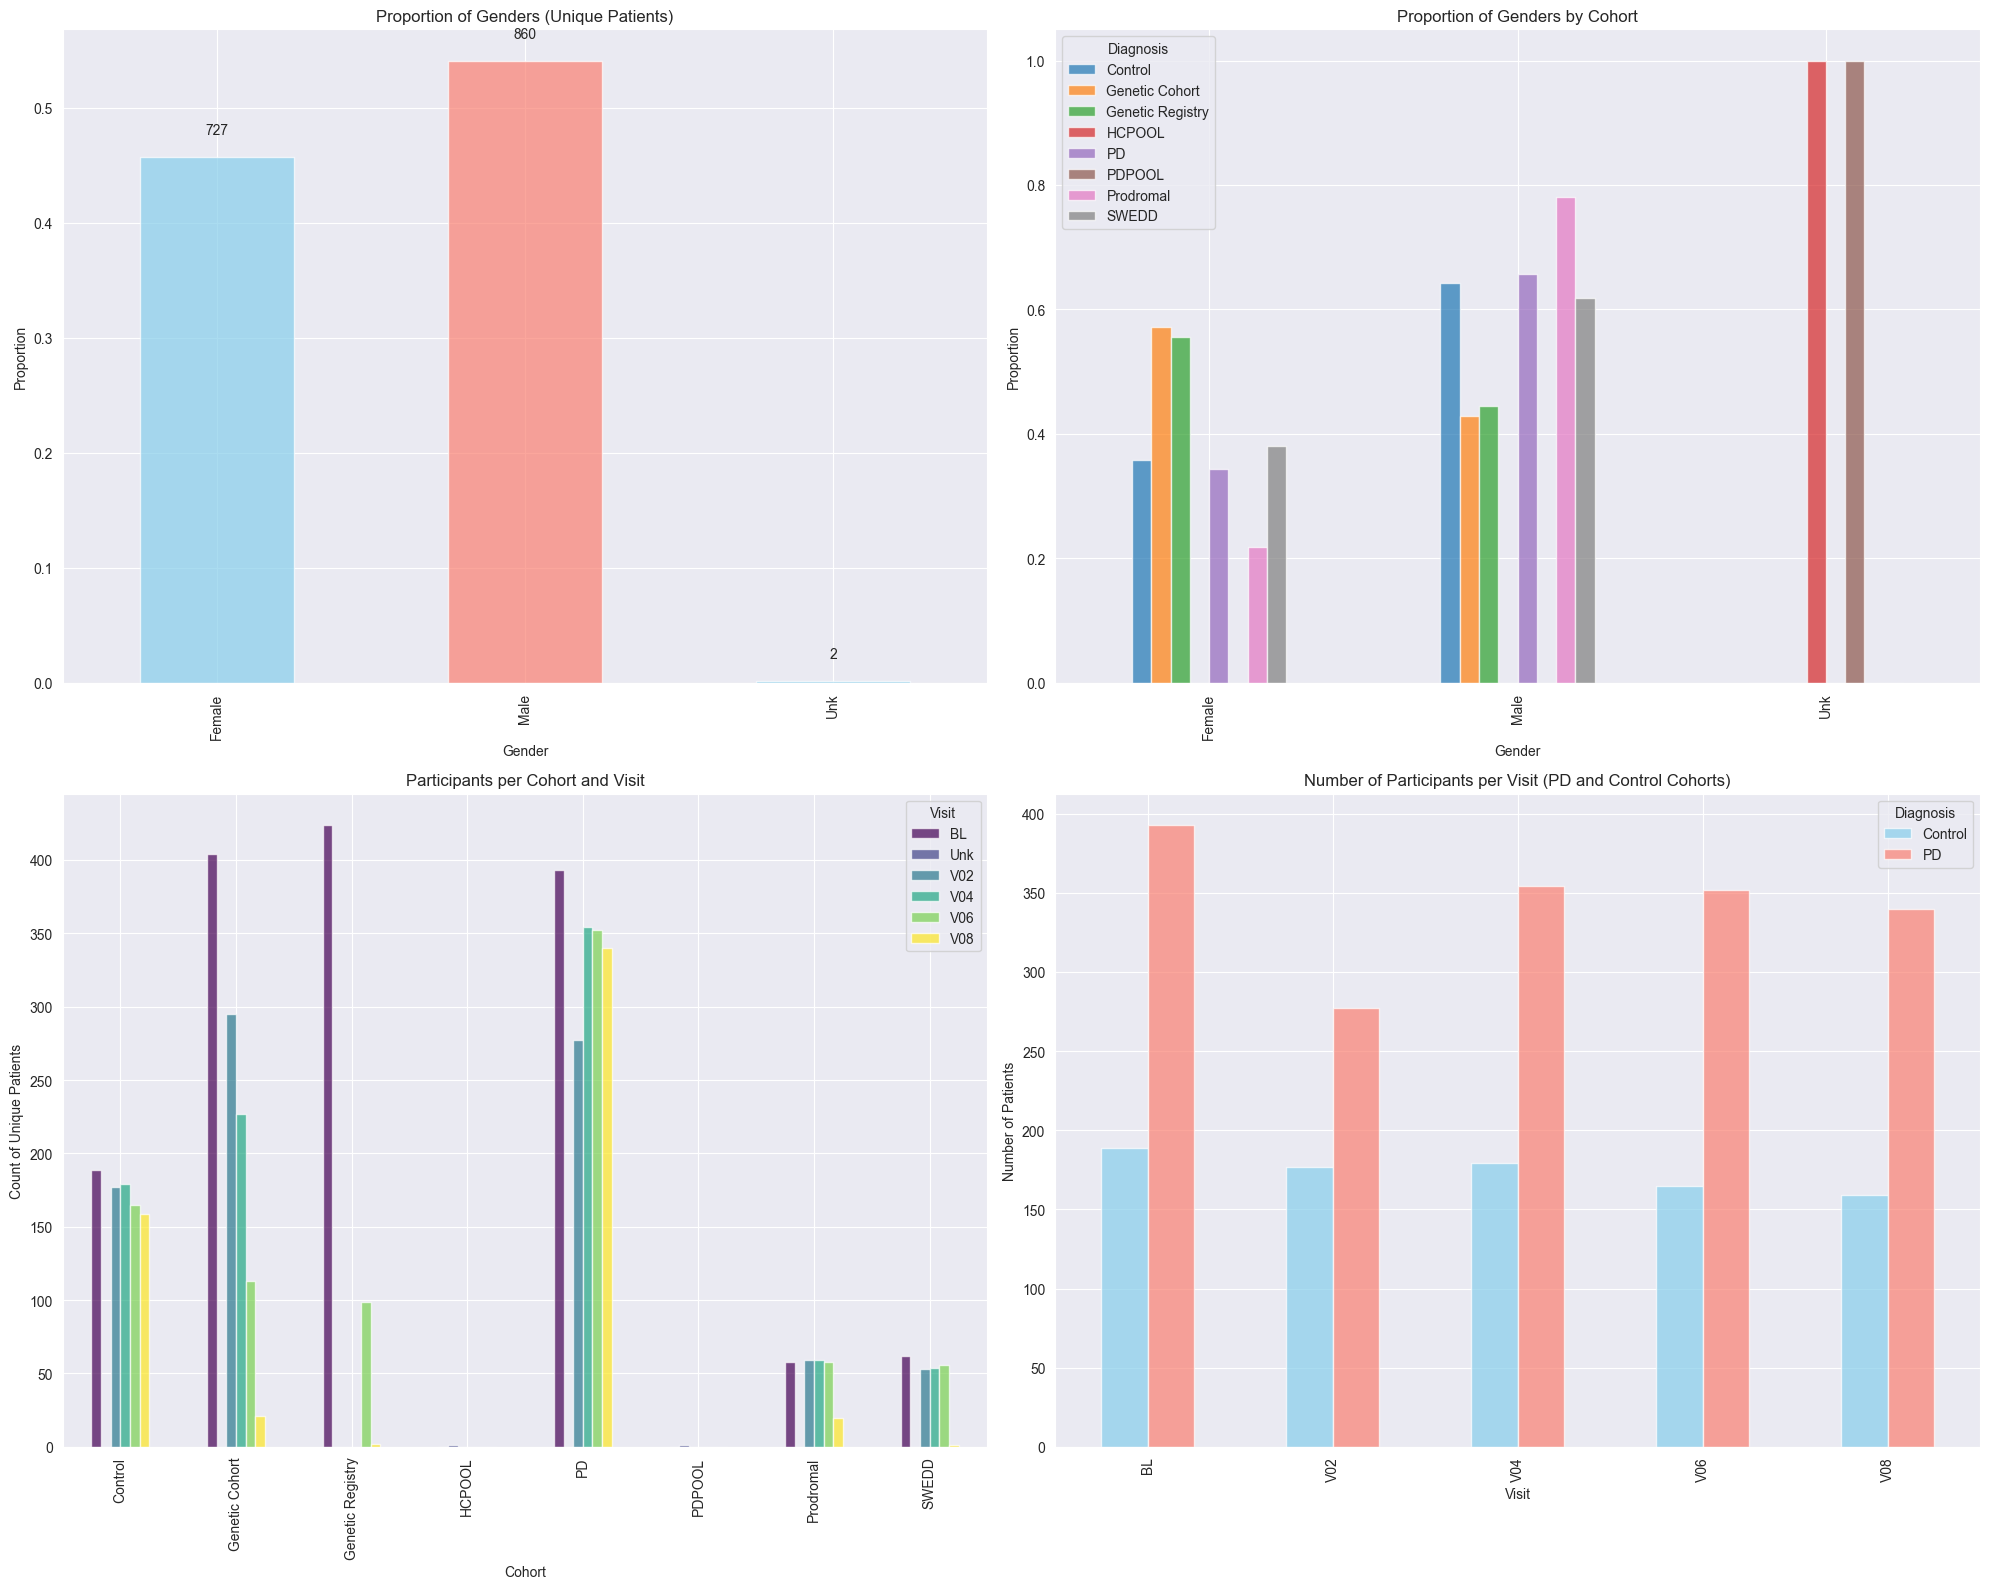
\includegraphics[width=0.73\linewidth]{Chapter-2-Section-2.1/ppmi-prop-gender-abs-per-cohort_samples-per-coh-visit-all-coh_pd-vs-ctrl.png}
                \caption[Πλήθος συμμετέχοντων ανά φύλο]{Επάνω αριστερά: Συμμετέχοντες ανά φύλο συνολικα, Επάνω δεξιά: Συμμετέχοντες ανά ομάδα. Κάτω αριστερά: Συμμετέχοντες ανά ομάδα και επίσκεψη. Κάτω δεξιά: Συμμετέχοντες ανά ομάδα και επίσκεψη.}
                \label{fig:ppmi-proportion-of-genders-absolute-and-per-cohort}
            \end{figure}
        \par
            Πρέπει να σημειωθεί ότι η αλληλούχιση διενεργήθηκε σε δύο διαφορετικές φάσεις. Αυτό δεν σημαίνει πως η δειγματοληψία ακολούθησε επίσης αυτόν τον διαχωρισμό, έτσι ώστε να προκύψουν για κάθε συμμετέχοντα δέκα δείγματα, ήτοι πέντε επισκέψεις επί δύο φάσεις, αλλά δείγματα από τις πέντε (\emph{ή και λιγότερες}) διαφορετικές επισκέψεις μπορεί να αλληλουχίστηκαν σε διαφορετικές φάσεις. Σαφώς αυτό καθιστά έναν τεχνικό παράγοντα που μπορεί να οδηγήσει σε ανακριβή αποτελέσματα σε αναλύσεις. Ειδικά η αλληλούχιση των δειγμάτων της δεύτερης επίσκεψης έχει γίνει αποκλειστικά στη δεύτερη φάση, σύμφωνα με την εικόνα~\ref{fig:ppmi-bars-pd-ctrl-visits-per-phase}. Ένα επίσης ερώτημα μπορεί να απαντηθεί ως προς το αν τα δείγματα όλων των ηλικιακών ομάδων εκπροσωπούνται και στις δύο φάσεις. Με το γράφημα στην εικόνα~\ref{fig:ppmi-bars-pd-ctrl-age_groups-per-phase} η απάντηση μπορεί να δοθεί καταφατικά, όπως επίσης και ότι δεν υπάρχει αξιοσημείωτη ασυμμετρία στην κατανομή των ηλικιακών ομάδων ανά φάση αλληλούχισης.

            \begin{figure}[ht]
                \centering
                \begin{subfigure}[b]{0.48\textwidth}
                    \centering
                    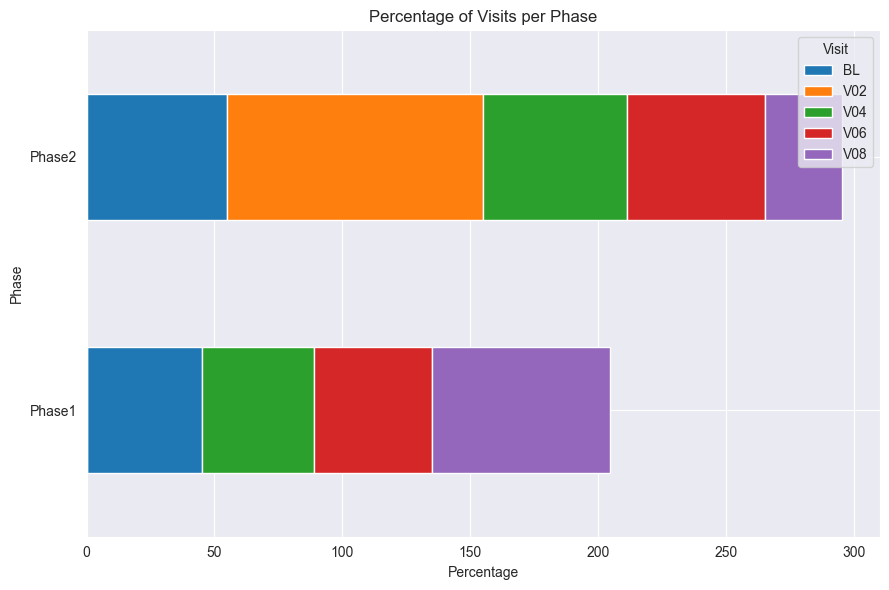
\includegraphics[width=\linewidth,height=7.5cm]{Chapter-2-Section-2.1/ppmi-bars-pd-ctrl-visits-per-phase.png}
                    \caption{Κατανομή δειγμάτων ανά επίσκεψη και φάση αλληλούχισης}
                    \label{fig:ppmi-bars-pd-ctrl-visits-per-phase}
                \end{subfigure}
                \hfill
                \begin{subfigure}[b]{0.48\textwidth}
                \centering
                    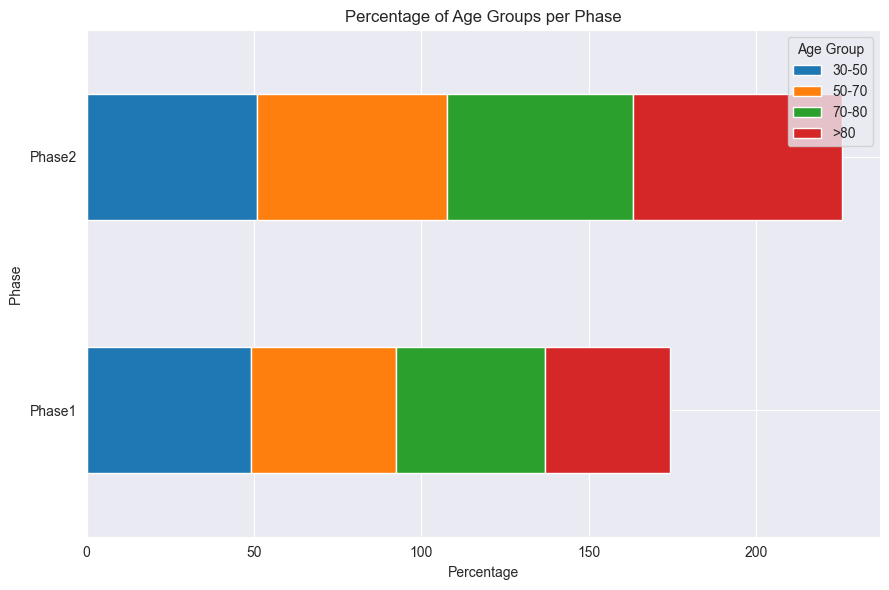
\includegraphics[width=\linewidth,height=7.5cm]{Chapter-2-Section-2.1/ppmi-bars-pd-ctrl-age_groups-per-phase.png}
                    \caption{Κατανομή ηλικιακών ομάδων ανά φάση αλληλούχισης}
                    \label{fig:ppmi-bars-pd-ctrl-age_groups-per-phase}
                \end{subfigure}
                \label{fig:ppmi-visit-phase-sample-distributions}
                \caption{Οπτικοποίηση δειγμάτων ανά φάση αλληλούχισης}
            \end{figure}
        \newpage

        \section{Ανάλυση κυρίων συνιστωσών}
            \par
                Στην εικόνα \ref{fig:ppmi-pca-pd-ctrl-all-visits-hue_diagnosis} παρουσιάζεται το αποτέλεσμα της PCA για τις πρώτες πέντε συνιστώσες όπου ο χρωματισμός πραγματοποιήθηκε σύμφωνα με τη διάγνωση. Δεν διακρίνονται ξεχωριστές συστάδες, γεγονός που συνιστά πως η μεταβλητότητα των εκφράσεων δεν διαχωρίζει σε αυτό το επίπεδο ανάλυσης δείγματα νοσούντων από υγιείς. Ενδιαφέρουσα είναι η απεικόνιση κυρίων συνιστωσών με χρωματισμό με βάση το φύλο, όπου διακρίνονται συστάδες μεταξύ της πέμπτης συνιστώσας και όλων των υπολοίπων. Το συμπέρασμα είναι, πως υπάρχει μεταβλητότητα σύμφωνα με γονιδιακές εκφράσεις στα δείγματα ολικού αίματος με την οποία δύναται να διακριθούν τα δείγματα των δύο φύλων. Πρόκειται για πολύ μικρό μέρος εκ του συνόλου της μεταβλητότητας (\emph{Πίνακας~\ref{tab:pca}}). Η στρωμάτωση των δειγμάτων σε παρακάτω βήματα χρησιμεύει προς αποφυγήν της όποιας πιθανής παρεμβολής στις διάφορες αναλύσεις.

            \begin{figure}[ht]
                \centering
                \begin{subfigure}[b]{0.48\textwidth}
                    \centering
                    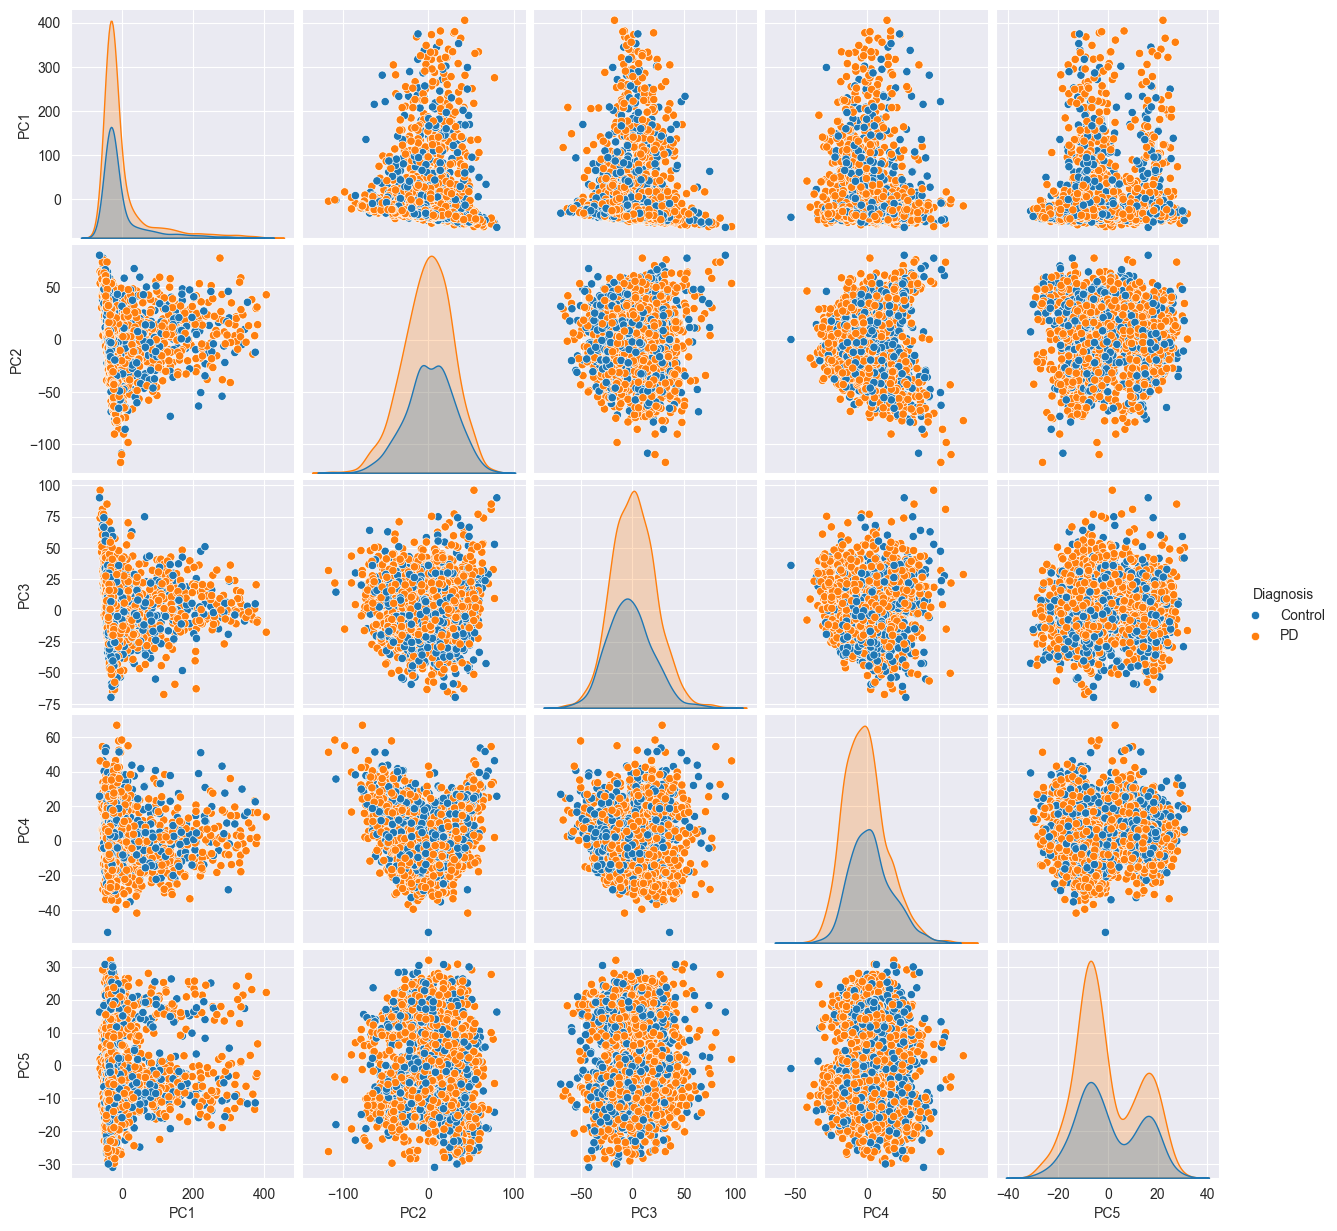
\includegraphics[width=\linewidth,height=7cm]{Chapter-2-Section-2.1/ppmi-pca-pd-ctrl-all-visits-hue_diagnosis.png}
                    \caption{PCA σύμφωνα με την διάγνωση}
                    \label{fig:ppmi-pca-pd-ctrl-all-visits-hue_diagnosis}                
                \end{subfigure}
                \hfill
                \begin{subfigure}[b]{0.48\textwidth}
                    \centering
                    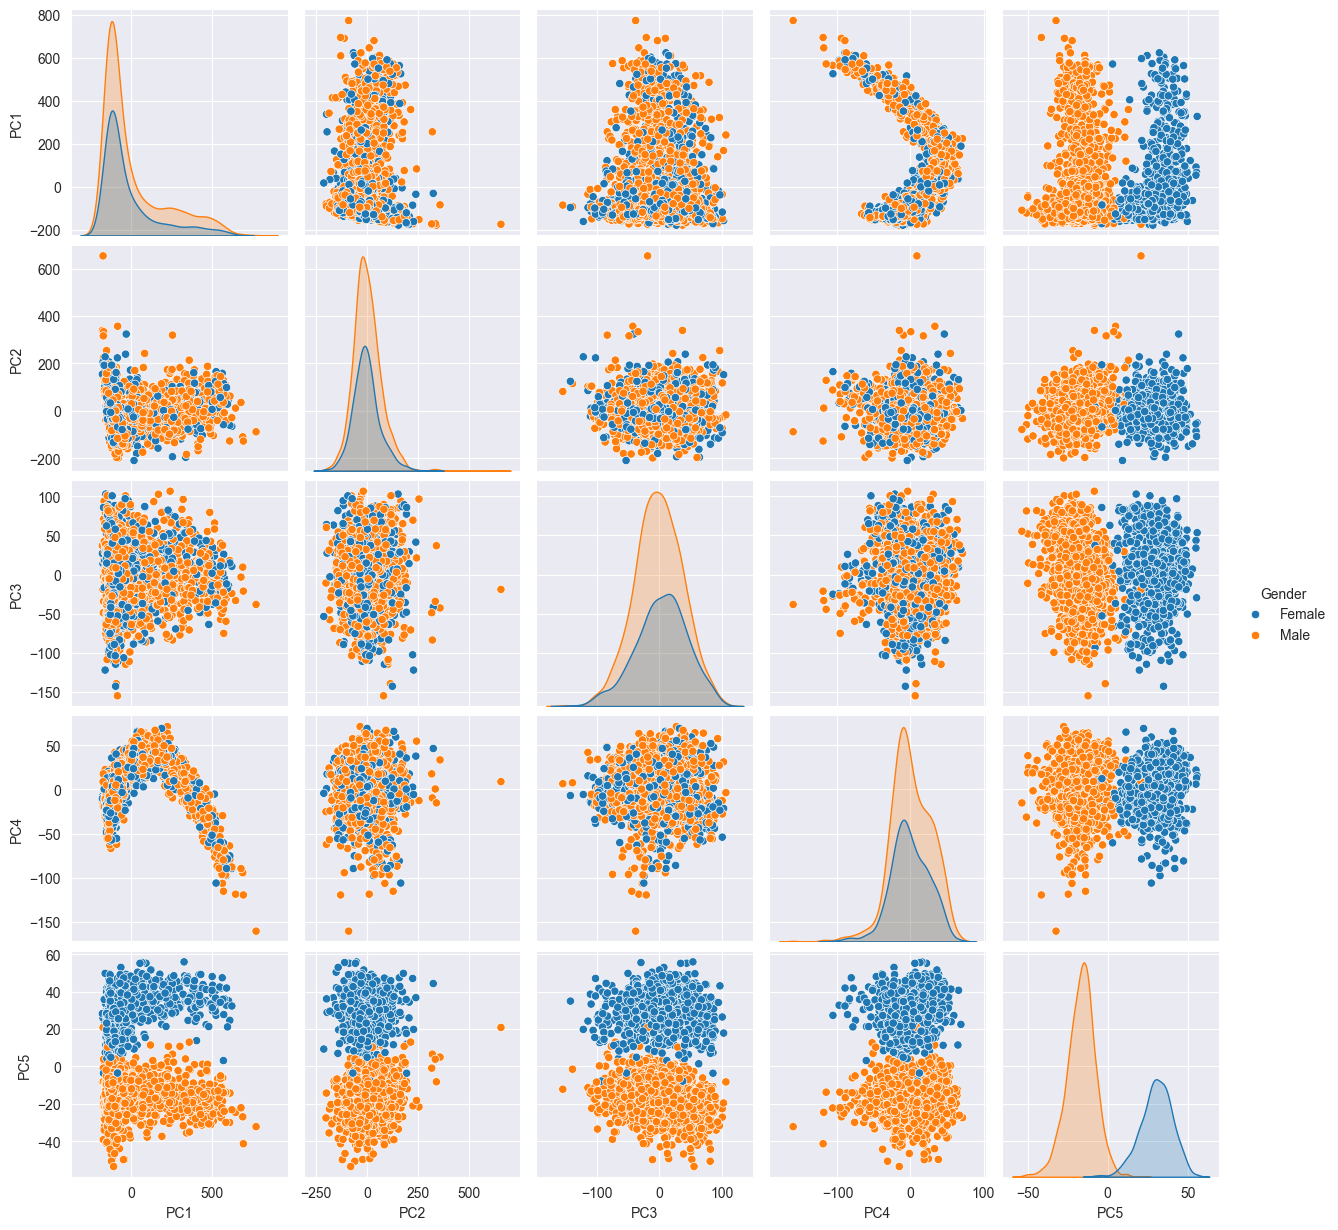
\includegraphics[width=\linewidth,height=7cm]{Chapter-2-Section-2.1/ppmi-pca-pd-ctrl-all-visits-hue_gender.png}
                    \caption{PCA σύμφωνα με τo φύλο}
                    \label{fig:ppmi-pca-pd-ctrl-all-visits-hue_gender}    
                \end{subfigure}
                \label{fig:ppmi-pca-scatterplot}
                \caption{Αποτελέσματα PCA}
            \end{figure}

            \begin{table}[ht]
                \centering
                \caption{Μεταβλητότητα ανά συνιστώσα}
                \begin{tabular}{lcccc} % No vertical lines
                    \toprule
                    \textbf{PC 1} & \textbf{PC 2} & \textbf{PC 3} & \textbf{PC 4} & \textbf{PC 5} \\
                    \midrule
                    56,88\% & 8,77\% & 5,15\% & 2,44\% & 1,78\% \\
                    \bottomrule
                \end{tabular}
                \label{tab:pca}
            \end{table}
            \newpage
            \par
                Παρακάτω απεικονίζεται το αποτέλεσμα της PCA σύμφωνα με τη φάση αλληλούχισης. Εντός των πρώτων πέντε κύριων συνιστωσών δεν παρατηρείται ομαδοποίηση και μαζί με αυτό προκύπτει και η διαβεβαίωση πως δεν εισάγεται τεχνικός θόρυβος από τη φάση αλληλούχισης.
                \begin{figure}[H]
                    \centering
                    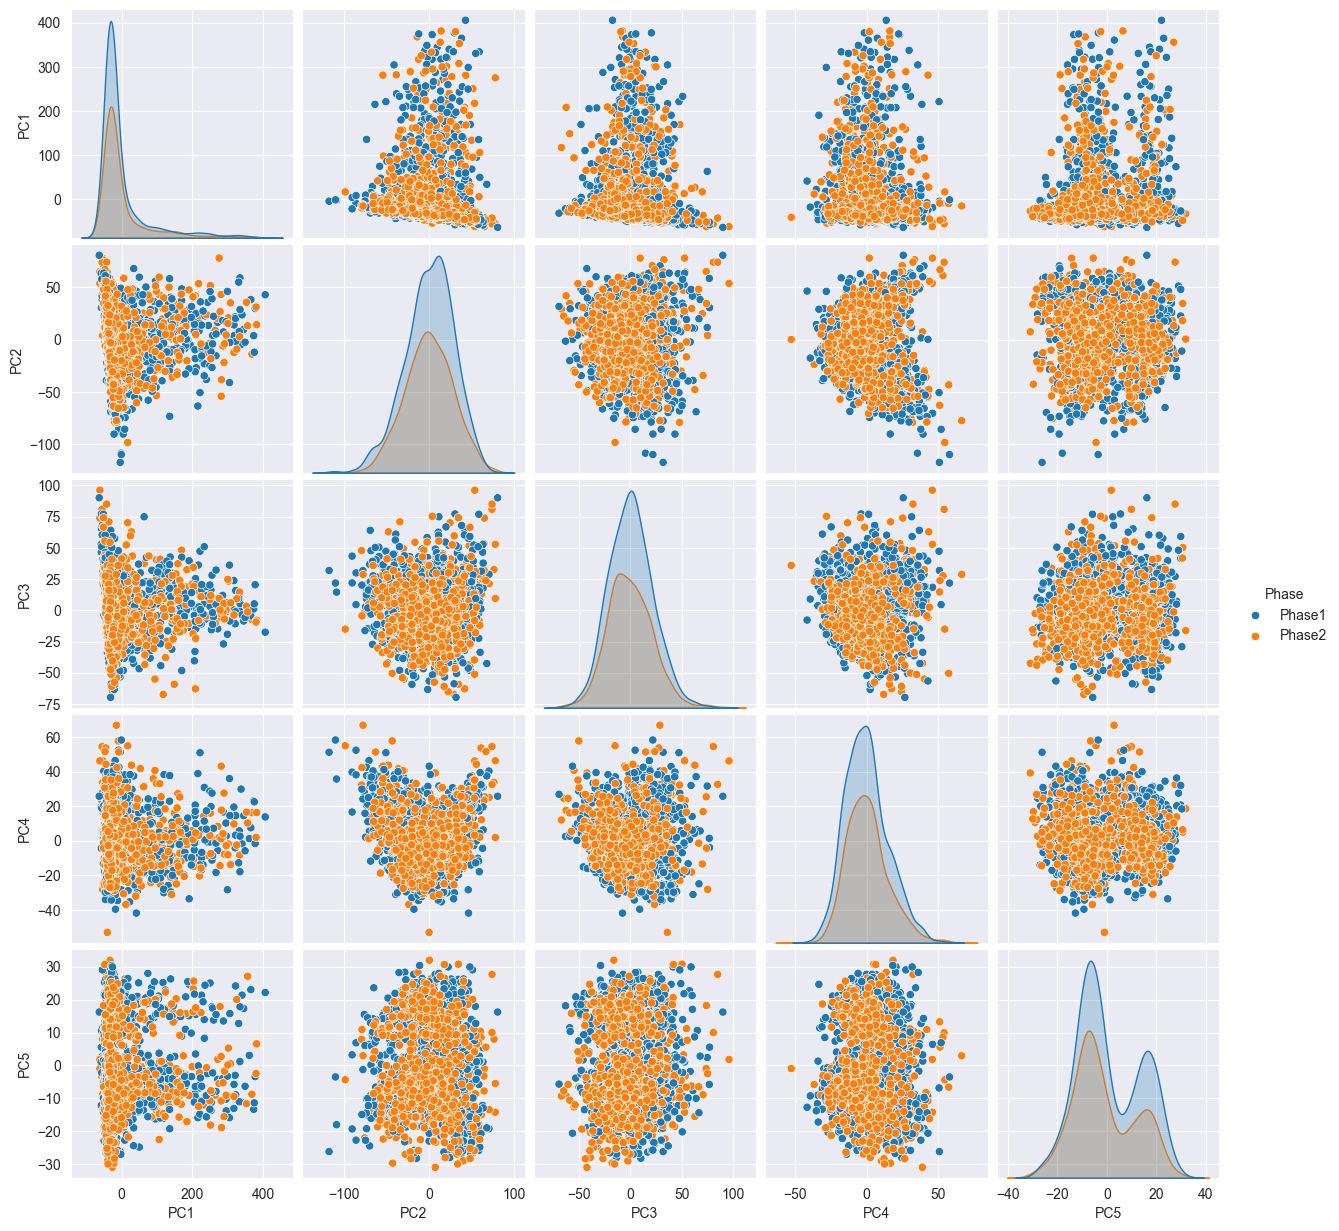
\includegraphics[width=0.75\textwidth]{Chapter-2-Section-2.1/ppmi-pca-pd-ctrl-all-visits-hue-phase.png}
                    \caption{PCA σύμφωνα με τη φάση αλληλούχισης}
                    \label{fig:ppmi-pca-pd-ctrl-all-visits-hue-phase}
                \end{figure}
    \section{Ανάλυση διαφορικής γονιδιακής έκφρασης}
        \par
            Η ανάλυση διαφορικής έκφρασης (\emph{DGEA\nomenclature{DGEA}{Differential Gene Expression Analysis}}) διενεργήθηκε μετά από στρωματοποίηση των δειγμάτων σύμφωνα με το φύλο και την ηλικιακή ομάδα με τη χρήση του πακέτου λογισμικού της R, DESeq2 (\emph{\cite{Love2014ModeratedDESeq2}}) (\emph{κώδικας~\ref{lst:mainr}}) και αντίστοιχη οπτικοποίηση με χρήση σεναρίου στην γλώσσα Python (\emph{κώδικας~\ref{lst:processdegconsolidatedvisitspy}}). Η επίσκεψη της κάθε δειγματοληψίας συμπεριλήφθηκε ως συμμεταβλητή και θεωρήθηκε ως τεχνικός παράγοντας, χωρίς να ερευνηθεί αν έχει βιολογικό χαρακτήρα ως προς την πρόοδο της νόσου. Ως όριο για την έκφραση $|log_2FoldChange|$ τέθηκε η τιμή $>0,5$ ενώ για την τιμή της $padj<0,05$.
        \par
            Το αντίστοιχο τμήμα της διαδικασίας ανάλυσης (\emph{Pipeline}) παρουσιάζεται στην εικόνα~\ref{fig:msci-big-pic-DEGs-blocks}. Το κομμάτι αυτό κατακερματίζει το σύνολο δεδομένων σύμφωνα με το φύλο και την ηλικιακή ομάδα των συμμετεχόντων σε υποσύνολα, όπου για κάθε υποσύνολο διεξάγεται η διαφορική ανάλυση μέσω DESeq2. Πέραν της διάγνωσης, συμπεριλήφθηκε και η παρατήρηση των επισκέψεων δειγματοληψίας (\emph{Visit}), καθώς καθιστά πηγή μεταβλητότητας η οποία πρέπει να ληφθεί υπόψη ως τεχνικός παράγοντας στην στατιστική ανάλυση (\emph{\cite{Love2016DifferentialPackage}}).
        \par
            Τα αποτελέσματα περιέχουν τα διαφορικά εκφραζόμενα και καταγράφονται σε μορφή CSV σε διαφορετικά αρχεία για περαιτέρω ανάλυση.
            \begin{figure}[h]
                \centering
                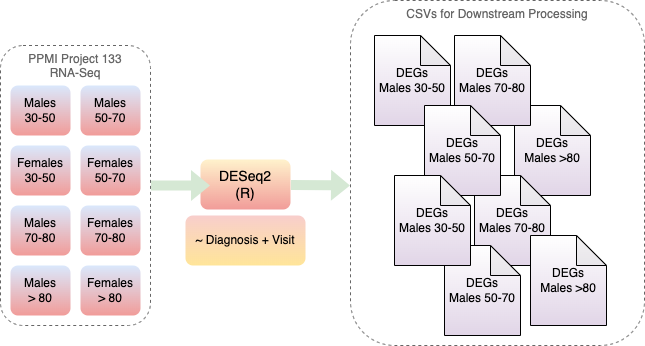
\includegraphics[width=0.7\textwidth]{Chapter-3/msci-big-pic-DEGs-blocks.png}
                \caption{Pipeline για την ανάλυση διαφορικής έκφρασης με εξαγωγή αποτελεσμάτων σε αρχεία CSV}
                \label{fig:msci-big-pic-DEGs-blocks}
            \end{figure}
        \subsection{Διαφορική έκφραση γονιδίων σε γυναίκες}
         \par
            Το πλήθος των στατιστικά σημαντικών εκφραζόμενων γονιδίων ποικίλει ανά ηλικιακή ομάδα. Στη σειρά διαγραμμάτων της εικόνας~\ref{fig:volcano_plot_consoVisits_Female} διακρίνονται περισσότερα γονίδια στατιστικής σημασίας στην ηλικιακή ομάδα 30-50 έναντι της ομάδας 50-70 ετών. Ενδεχομένως η νόσος να διαφοροποιείται σε γονιδιακό επίπεδο σε περιπτώσεις όπου η νόσος εκδηλώνεται σε μικρότερες ηλικίες. Σε ηλικίες άνω των 70 ετών το πλήθος των διαφορικά εκφραζόμενων γονιδίων στατιστικής σημασίας αυξάνεται σημαντικά, κάτι που μπορεί να παραπέμπει και στην πρόοδο της νόσου με αυξανόμενη ηλικία. Όσον αφορά το πλήθος των υπέρ-έναντι των υπό-εκφραζόμενων γονιδίων, ισχύει σύμφωνα με την παρακάτω οπτικοποίηση στην εικόνα~\ref{fig:barplot_plot_consoVisits_Female}, ότι υπάρχουν περισσότερα υπέρ-εκφραζόμενα γονίδια σε όλες τις ηλικιακές ομάδες υπό παρατήρηση.
            \begin{figure}[h]
                \centering
                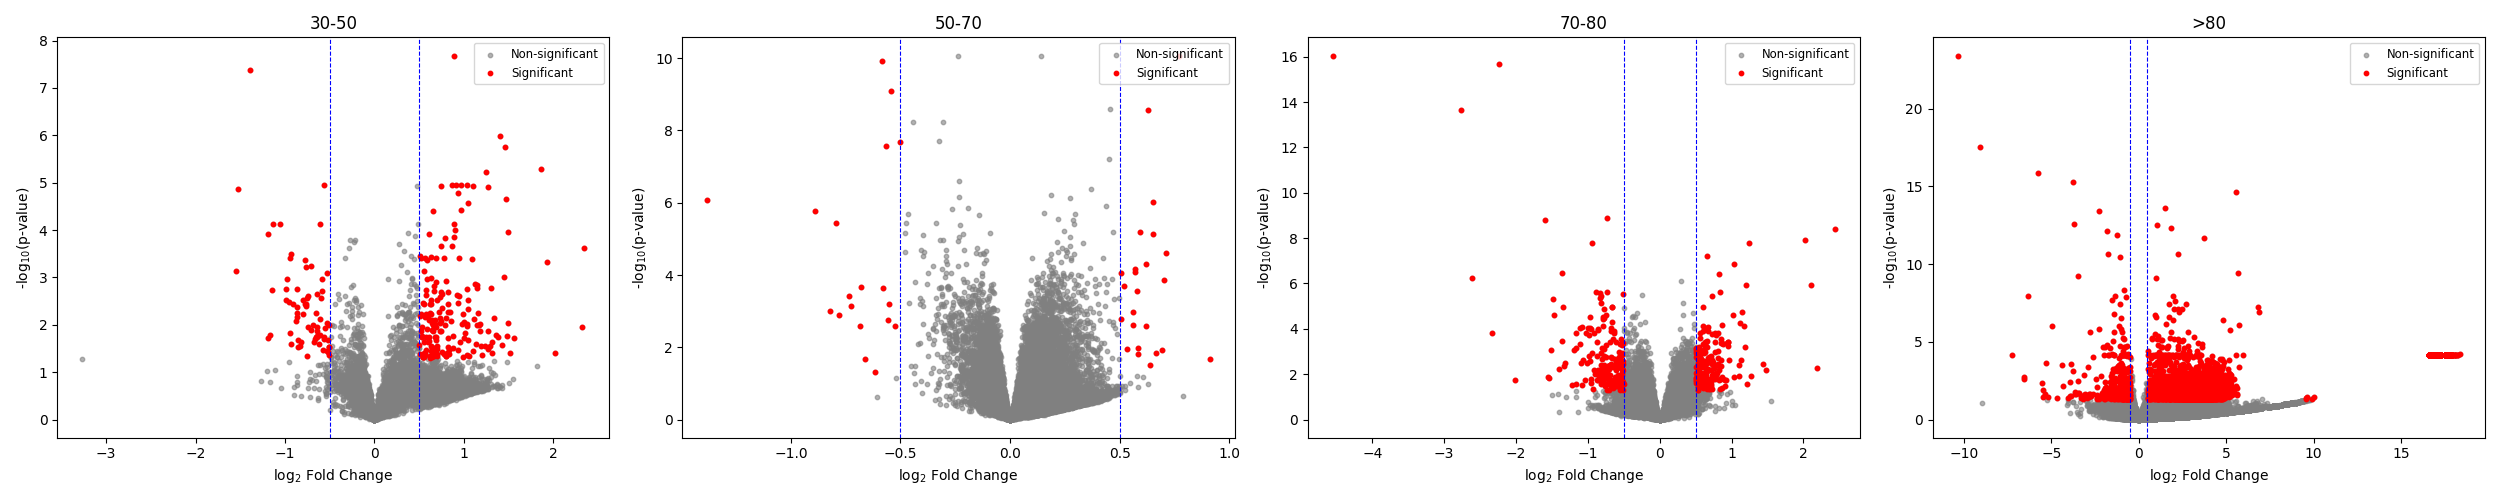
\includegraphics[width=\textwidth,height=4cm]{Chapter-3/volcano_plot_consoVisits_Female.png}
                \caption{Διαγράμματα Ηφαιστείου ανά ηλικιακή ομάδα γυναικών}
                \label{fig:volcano_plot_consoVisits_Female}
            \end{figure}
            \begin{figure}[H]
                \centering
                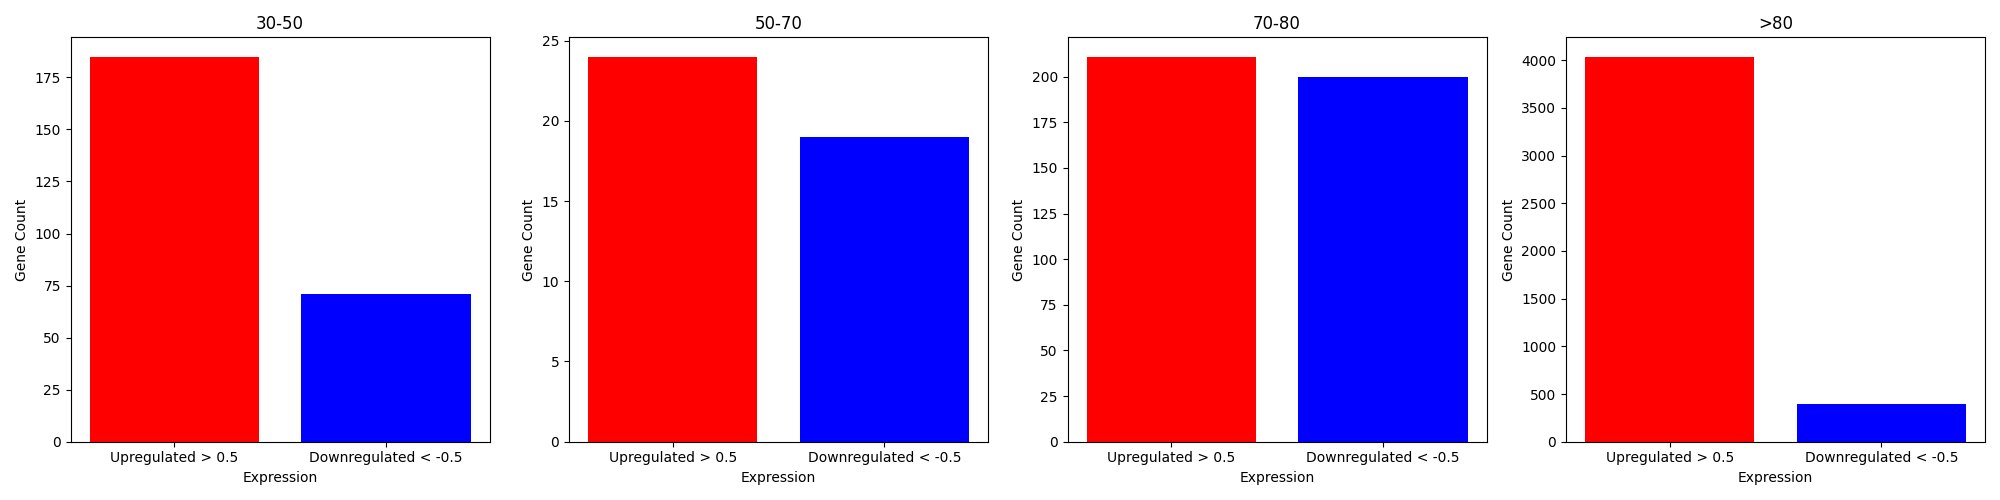
\includegraphics[width=\textwidth,height=4cm]{Chapter-3/barplot_plot_consoVisits_Female.png}
                \caption{Πλήθος στατιστικά σημαντικών διαφορικά εκφραζόμενων γονιδίων - Γυναίκες}
                \label{fig:barplot_plot_consoVisits_Female}
            \end{figure}

        \subsection{Διαφορική έκφραση γονιδίων σε άνδρες}
        \par
            Συνολικά η διαφορική έκφραση γονιδίων στους άνδρες σε κάθε ηλικιακή ομάδα διαφέρει από τις εκφράσεις των γυναικών. Χαρακτηριστική είναι η παρουσία περισσότερων υπέρ-εκφραζόμενων γονιδίων έναντι ελάχιστων υπό-εκφραζόμενων στην ηλικιακή ομάδα των 50-70, ενώ στις υπόλοιπες περιπτώσεις ο αριθμός των υπό-εκφραζόμενων δείχνει να είναι περίπου διπλάσιος από των υπέρ-εκφραζόμενων.
            \begin{figure}[h]
                \centering
                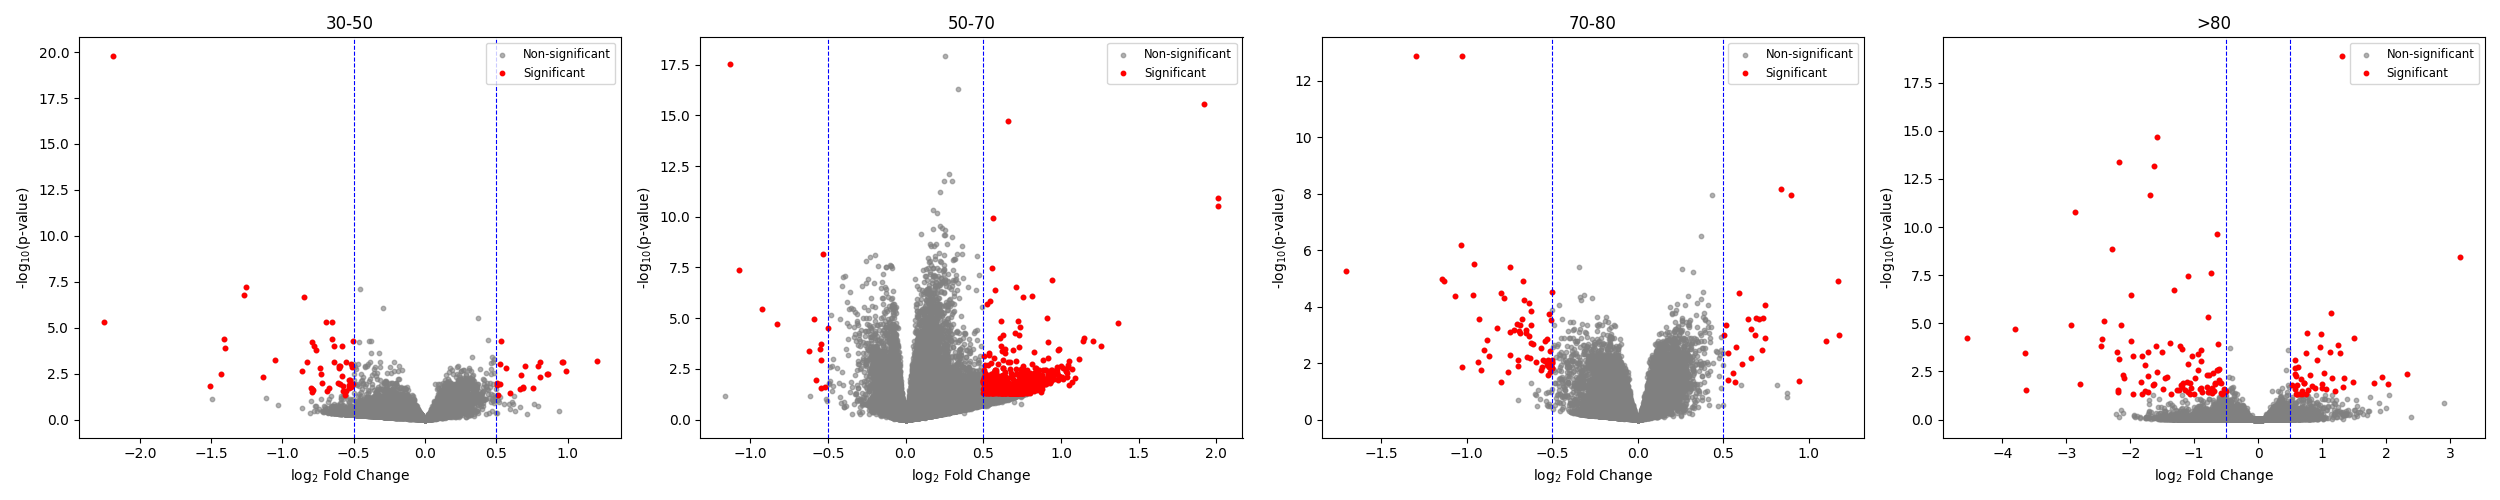
\includegraphics[width=\textwidth,height=4cm]{Chapter-3/volcano_plot_consoVisits_Male.png}
                \caption{Διαγράμματα Ηφαιστείου ανά ηλικιακή ομάδα ανδρών}
                \label{fig:volcano_plot_consoVisits_Male}
            \end{figure}
            \begin{figure}[H]
                \centering
                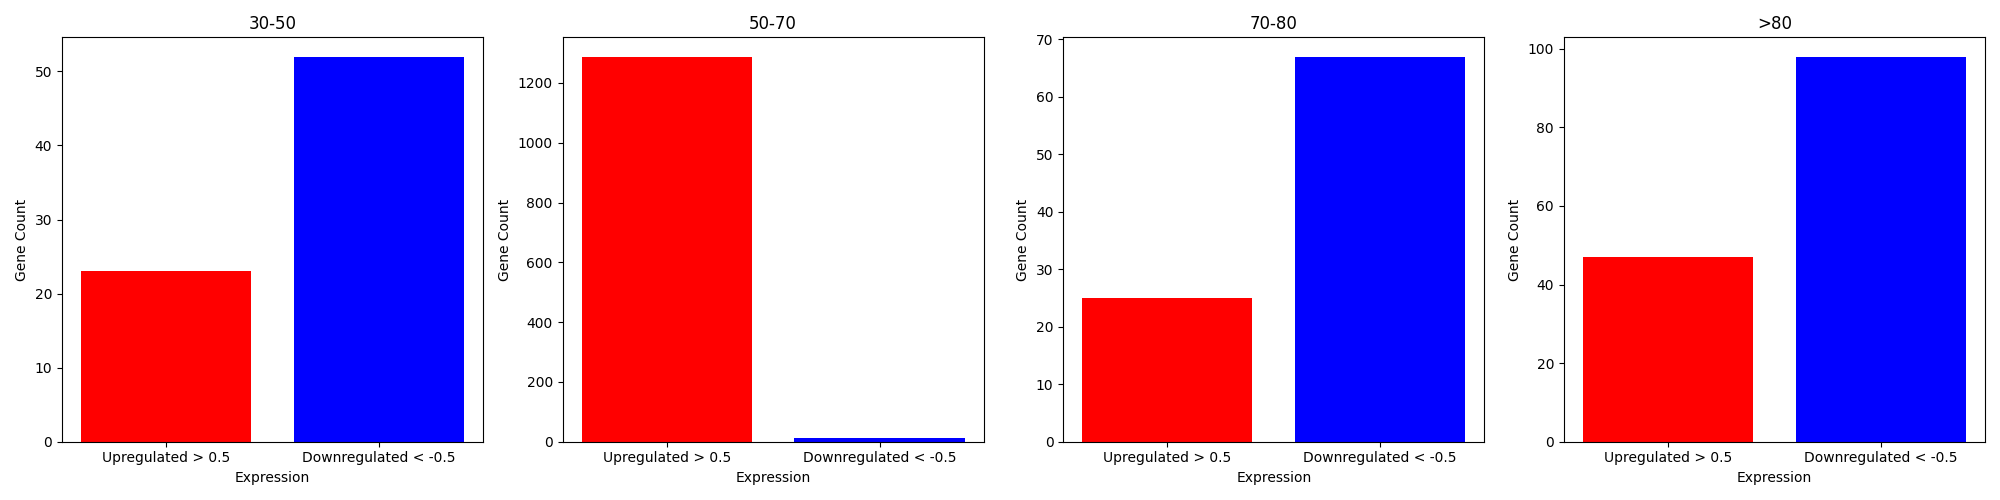
\includegraphics[width=\textwidth,height=4cm]{Chapter-3/barplot_plot_consoVisits_Male.png}
                \caption{Πλήθος στατιστικά σημαντικών διαφορικά εκφραζόμενων γονιδίων - Άνδρες}
                \label{fig:barplot_plot_consoVisits_Male}
            \end{figure}
        \subsection{Σύνοψη της ανάλυσης διαφορικής έκφρασης}
            \par
                Τα αποτελέσματα ανά φύλο και ηλικιακή ομάδα διαφέρουν σε αριθμούς υπό- και υπέρ-εκφραζόμενων γονιδίων. Μια σύντομη σύνοψη των πρώτων έξι διαφορικά εκφραζόμενων γονιδίων παρουσιάζεται στον πίνακα~\ref{tab:top-6-degs-strata}. Πρόκειται για τα γονίδια που έχουν τις χαμηλότερες τιμές $padj$ καθώς και τις υψηλότερες απόλυτες τιμές $log_2FoldChange$.
                \begin{table}[ht]
                    \centering
                    \caption[Ενδεικτική επιλογή έξι διαφορικά εκφραζόμενων γονιδίων] {Ενδεικτική επιλογή έξι διαφορικά εκφραζόμενων γονιδίων με υψηλότερη απόλυτη τιμή έκφρασης και υψηλή στατιστική σημαντικότητα. Υπέρ-εκφραζόμενα γονίδια παρουσιάζονται με κόκκινο φόντο, υπό-εκφραζόμενα με μπλε. Κοινά γονίδια παρουσιάζονται \textbf{έντονα} και \underline{υπογραμμισμένα}}
                    \small
                    \setlength{\tabcolsep}{5pt}
                    \renewcommand{\arraystretch}{1.4}
                    \begin{tabular}{@{}>{\raggedright}p{1.3cm}cccc@{}}
                        \toprule
                        \textbf{Φύλο} & \textbf{30-50} & \textbf{50-70} & \textbf{70-80} & \textbf{>80} \\
                        \midrule
                        \multirow{6}{*}{'Ανδρες}
                        & \cellcolor{blue!20}\textbf{\underline{RNU671-P}} & \cellcolor{red!20}NFYAP1 & \cellcolor{blue!20}\textbf{\underline{RNU1-67P}} & \cellcolor{blue!20}LINC02506 \\
                        & \cellcolor{blue!20}CNTNAP3P2 & \cellcolor{red!20}ENSG00000270962 & \cellcolor{blue!20}NECTIN2 & \cellcolor{blue!20}ENSG00000276345 \\
                        & \cellcolor{blue!20}RNU1-83P & \cellcolor{red!20}LINC00355 & \cellcolor{red!20}\textbf{\underline{ENSG00000259385}} & \cellcolor{blue!20}DEFA3 \\
                        & \cellcolor{blue!20}TUSC3 & \cellcolor{red!20}TRIM64 & \cellcolor{red!20}LRRC37A2 & \cellcolor{blue!20}\textbf{\underline{ENSG00000223779}} \\
                        & \cellcolor{blue!20}LINC02470 & \cellcolor{red!20}ANKRD33BP9 & \cellcolor{blue!20}IFI44L & \cellcolor{red!20}\textbf{\underline{HLA-DQA2}} \\
                        & \cellcolor{blue!20}TUBB2B & \cellcolor{red!20}LCEP2 & \cellcolor{blue!20}CYP4F29P & \cellcolor{blue!20}PAX8-AS1 \\
                        \midrule
                        \multirow{6}{*}{Γυναίκες}
                        & \cellcolor{red!20}RNVU1-7 & \cellcolor{blue!20}\textbf{\underline{RNU1-67P}} & \cellcolor{blue!20}DCLRE1CP1 & \cellcolor{red!20}REXO1L10P \\
                        & \cellcolor{red!20}CTAG2 & \cellcolor{red!20}ADAD1P1 & \cellcolor{blue!20}LINC02899 & \cellcolor{red!20}MIR4289 \\
                        & \cellcolor{red!20}ADGRG7 & \cellcolor{blue!20}RAP1GAP & \cellcolor{blue!20}\textbf{\underline{HLA-DQA2}} & \cellcolor{red!20}ENSG00000241573 \\
                        & \cellcolor{red!20}MRPS35-DT & \cellcolor{blue!20}\textbf{\underline{ENSG00000259385}} & \cellcolor{red!20}C4BPA & \cellcolor{red!20}IQCJ-SCHIP1-AS1 \\
                        & \cellcolor{red!20}ENSG00000275649 & \cellcolor{blue!20}ENSG00000265218 & \cellcolor{blue!20}CEACAMP3 & \cellcolor{red!20}ENSG00000238140 \\
                        & \cellcolor{red!20}\textbf{\underline{ENSG00000223779}} & \cellcolor{blue!20}CTXN2-AS1 & \cellcolor{blue!20}AGAP12P & \cellcolor{red!20}ENSG00000236046 \\
                        
                        \bottomrule
                    \end{tabular}
                    \label{tab:top-6-degs-strata}
                \end{table}
                \par
                    Στην εικόνα~\ref{fig:common-genes-across-genders-per-age-group} παρατίθενται στα εξής διαγράμματα κοινά γονίδια μεταξύ των φύλων ανά ηλικιακή ομάδα, στατιστικά σημαντικά και με τιμές έκφρασης $|log_2FoldChange| > 0,5$. Από τα κοινά γονίδια υπάρχουν μόνο λίγα που παρουσιάζουν ίδιο πρότυπο έκφρασης, δηλαδή είτε και στα δυο φύλα να υπέρ- ή να υπό-εκφράζονται.
                    \begin{figure}[ht]
                        \centering
                        \begin{subfigure}[b]{0.48\textwidth}
                            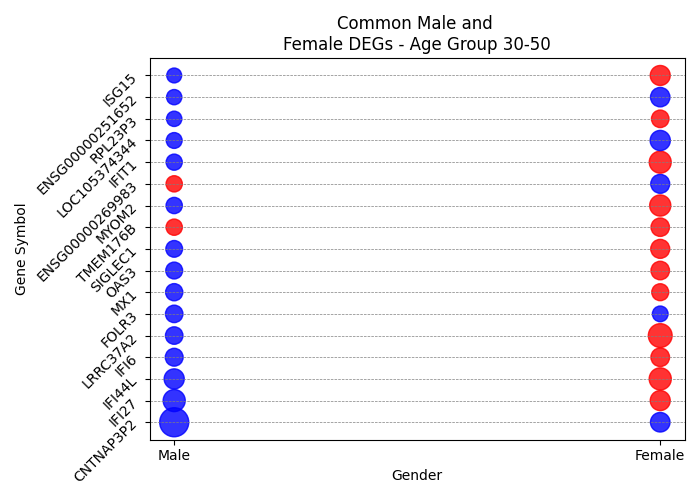
\includegraphics[width=\textwidth]{Chapter-3/bubbleplot_combined_30-50.png}
                            \caption{Κοινά διαφορικά εκφραζόμενα γονίδια ηλικίας 30-50}
                            \label{fig:bubbleplot_combined_30-50}
                        \end{subfigure}
                        \hfill % Add horizontal fill
                        \begin{subfigure}[b]{0.48\textwidth}
                            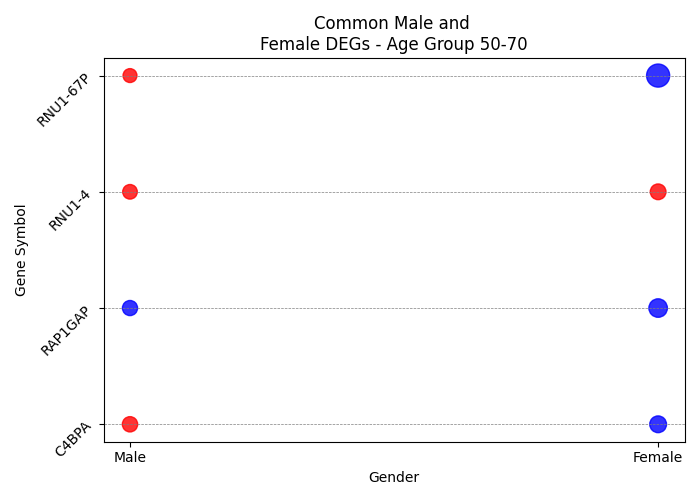
\includegraphics[width=\textwidth]{Chapter-3/bubbleplot_combined_50-70.png}
                            \caption{Κοινά διαφορικά εκφραζόμενα γονίδια ηλικίας 50-70}
                            \label{fig:bubbleplot_combined_50-70}
                        \end{subfigure}
                        
                        \vspace{0.5cm} % Vertical spacing between rows
                        
                        \begin{subfigure}[b]{0.48\textwidth}
                            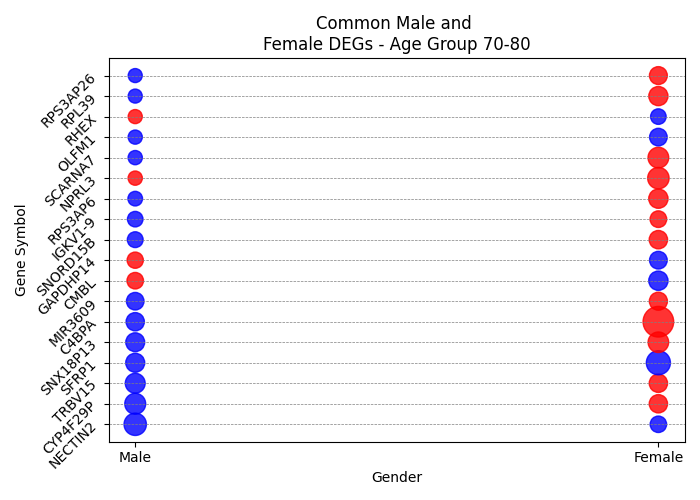
\includegraphics[width=\textwidth]{Chapter-3/bubbleplot_combined_70-80.png}
                            \caption{Κοινά διαφορικά εκφραζόμενα γονίδια ηλικίας 70-80}
                            \label{fig:bubbleplot_combined_70-80}
                        \end{subfigure}
                        \hfill
                        \begin{subfigure}[b]{0.48\textwidth}
                            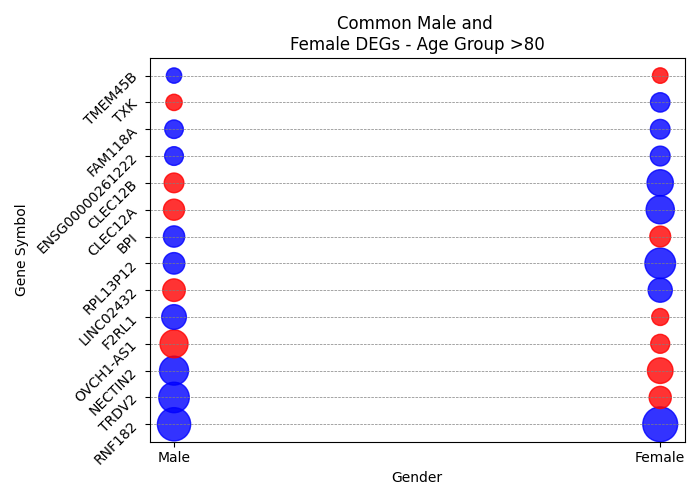
\includegraphics[width=\textwidth]{Chapter-3/bubbleplot_combined_>80.png}
                            \caption{Κοινά διαφορικά εκφραζόμενα γονίδια ηλικίας >80}
                            \label{fig:bubbleplot_combined_>80}
                        \end{subfigure}
                        
                        \caption{Κοινά διαφορικά εκφραζόμενα γονίδια μεταξύ ανδρών και γυναικών}
                        \label{fig:common-genes-across-genders-per-age-group}
                    \end{figure}
                \newpage
                \par    
                    Με μια σύντομη αναζήτηση στη βάση Gene4PD\footnote{http://genemed.tech/gene4pd}(\emph{\cite{Li2021Gene4PD:Disease}}), μιας βάσης δεδομένων στο διαδίκτυο για την αναζήτηση γενετικών πληροφοριών σχετικά με τη νόσο του Πάρκινσον, ανέκυψαν αποτελέσματα τα οποία συνοψίζονται στον πίνακα~\ref{tab:gene4pd-known-genes}.

                    \begin{table}[ht]
                        \centering
                        \small
                        % \setlength{\tabcolsep}{5pt}
                        % \renewcommand{\arraystretch}{1.4}
                        \begin{tabular}{cc}
                            \textbf{Ηλικιακή ομάδα} & \textbf{Γονίδιο} \\
                            \midrule
                             \multirow{2}{*}{30-50} & IF27\tablefootnote{http://genemed.tech/gene4pd/geneDetail/main?gene\_symbol=IFI27} \\
                             & MYOM2\tablefootnote{http://genemed.tech/gene4pd/geneDetail/main?gene\_symbol=MYOM2} \\
                             \midrule
                             50-70 & - \\
                             \midrule
                             \multirow{5}{*}{70-80} & RPL39\tablefootnote{http://genemed.tech/gene4pd/geneDetail/main?gene\_symbol=RPL39} \\
                             & NECTIN2\tablefootnote{http://genemed.tech/gene4pd/geneDetail/main?gene\_symbol=NECTIN2} \\
                             & OLFM1\tablefootnote{http://genemed.tech/gene4pd/geneDetail/main?gene\_symbol=OLFM1} \\
                             & CMBL\tablefootnote{http://genemed.tech/gene4pd/geneDetail/main?gene\_symbol=CMBL} \\
                             & SFRP1\tablefootnote{http://genemed.tech/gene4pd/geneDetail/main?gene\_symbol=SFRP1} \\
                             \midrule
                             \multirow{2}{*}{>80} & TXK\tablefootnote{http://genemed.tech/gene4pd/geneDetail/main?gene\_symbol=TXK} \\
                             & NECTIN2 \\
                        \end{tabular}
                        \caption{Γονίδια σχετικά με την νόσο του Πάρκινσον σύμφωνα με Gene4PD}
                        \label{tab:gene4pd-known-genes}
                    \end{table}                    
        \newpage
    \section{Κατηγοριοποίηση δειγμάτων μέσω Μηχανικής Μάθησης}
        \par
            Με την χρήση των δεδομένων της διαφορικής ανάλυσης γονιδιακής έκφρασης εκπαιδεύτηκαν τέσσερις διαφορετικοί κατηγοριοποιητές εποπτευόμενης μάθησης. Χρησιμοποιήθηκαν οι αλγόριθμοι λογιστικής παλινδρόμησης, SVM\nomenclature{SVM}{Support Vector Machines}, Random Forest και XGBoost. Πρόκειται για αλγόριθμους που χρησιμοποιούνται, μεταξύ άλλων, στον τομέα της βιοπληροφορικής.
        \par
            Η εφαρμογή της κατηγοριοποίησης πραγματοποιήθηκε σε όλα τα στρώματα (\emph{strata}) του συνόλου δεδομένων. Ως αποτελέσματα για την αποτίμηση της επίδοσης του κάθε αλγορίθμου ανά στρώμα, χρησιμοποιήθηκαν καθιερωμένες μετρικές όπως ROC-AUC\nomenclature{ROC-AUC}{Receiver Operating Characteristic}\nomenclature{AUC}{Area Under the Curve}, PR-AUC\nomenclature{PR}{Precission Recall} καθώς και η ευαισθησία και η ειδικότητα της κατηγοριοποίησης κατά την εκτέλεση. Η εκπαίδευση λειτούργησε με τη χρήση ενός εύρους παραμέτρων (\emph{Hyperparameters}) μέσω των οποίων ο κατηγοριοποιητής της κάθε μεθόδου δοκιμάζει και αποφασίζει τον βέλτιστο συνδυασμό παραμέτρων μετά από δεκαπλάσια διασταυρούμενη επικύρωση (\emph{10-fold Cross Validation}). Ο έτσι παραμετροποιημένος βέλτιστος κατηγοριοποιητής εκπαιδεύεται και μετέπειτα δοκιμάζεται σε κατηγοριοποίηση επί του αντίστοιχου συνόλου. 
        \par
            Τα σύνολα εκπαίδευσης και εκτέλεσης είναι διαφορετικά, με το σύνολο εκπαίδευσης να επιλέγεται στο 80\% επί του συνόλου δεδομένων ανά στρώμα, όπως και επίσης δείγματα από τα ίδια άτομα δεν βρίσκονται και στα δυο σύνολα, κάτι που θα είχε ως αποτέλεσμα το φαινόμενο του Feature Leakage (\emph{\cite{Oosterhuis2024LocalPredictions}}) και θα παραποιούσε σημαντικά τις μετρικές καθώς και την έκβαση της κατηγοριοποίησης. Για την επίτευξη του διαχωρισμού έγινε χρήση της κλάσης GroupShuffleSplit στην Python, από το πακέτο scikit (\emph{\cite{Buitinck2013APIProject}}). 
        \par
            Καθώς τα δείγματα των νοσούντων είναι σε όλα τα στρώματα περίπου διπλάσια των υγιών, η κατηγοριοποίηση θα λάβει χώρα προς όφελος της πλειοψηφίας, εάν η ανισορροπία (\emph{Class imbalance}) είναι αρκετά υψηλή (\emph{εικόνα~\ref{fig:ppmi-visual-bar-class-imb}}). Ως λύση για το εν λόγω πρόβλημα χρησιμοποιήθηκε η τεχνική SMOTE\nomenclature{SMOTE}{Synthetic Minority Oversampling Technique} (\emph{\cite{Cemernek2024EffectsInterpretability}}) που παρέχεται από το πακέτο imblearn της Python (\emph{\cite{Lemaitre2016Imbalanced-learn:Learning}}). Με την τεχνική αυτή, η κλάση που αποτελεί την μειοψηφία λαμβάνει επιπρόσθετα συνθετικά δείγματα προς αντιστάθμιση της ανισορροπίας.

            \begin{figure}[H]
                \centering
                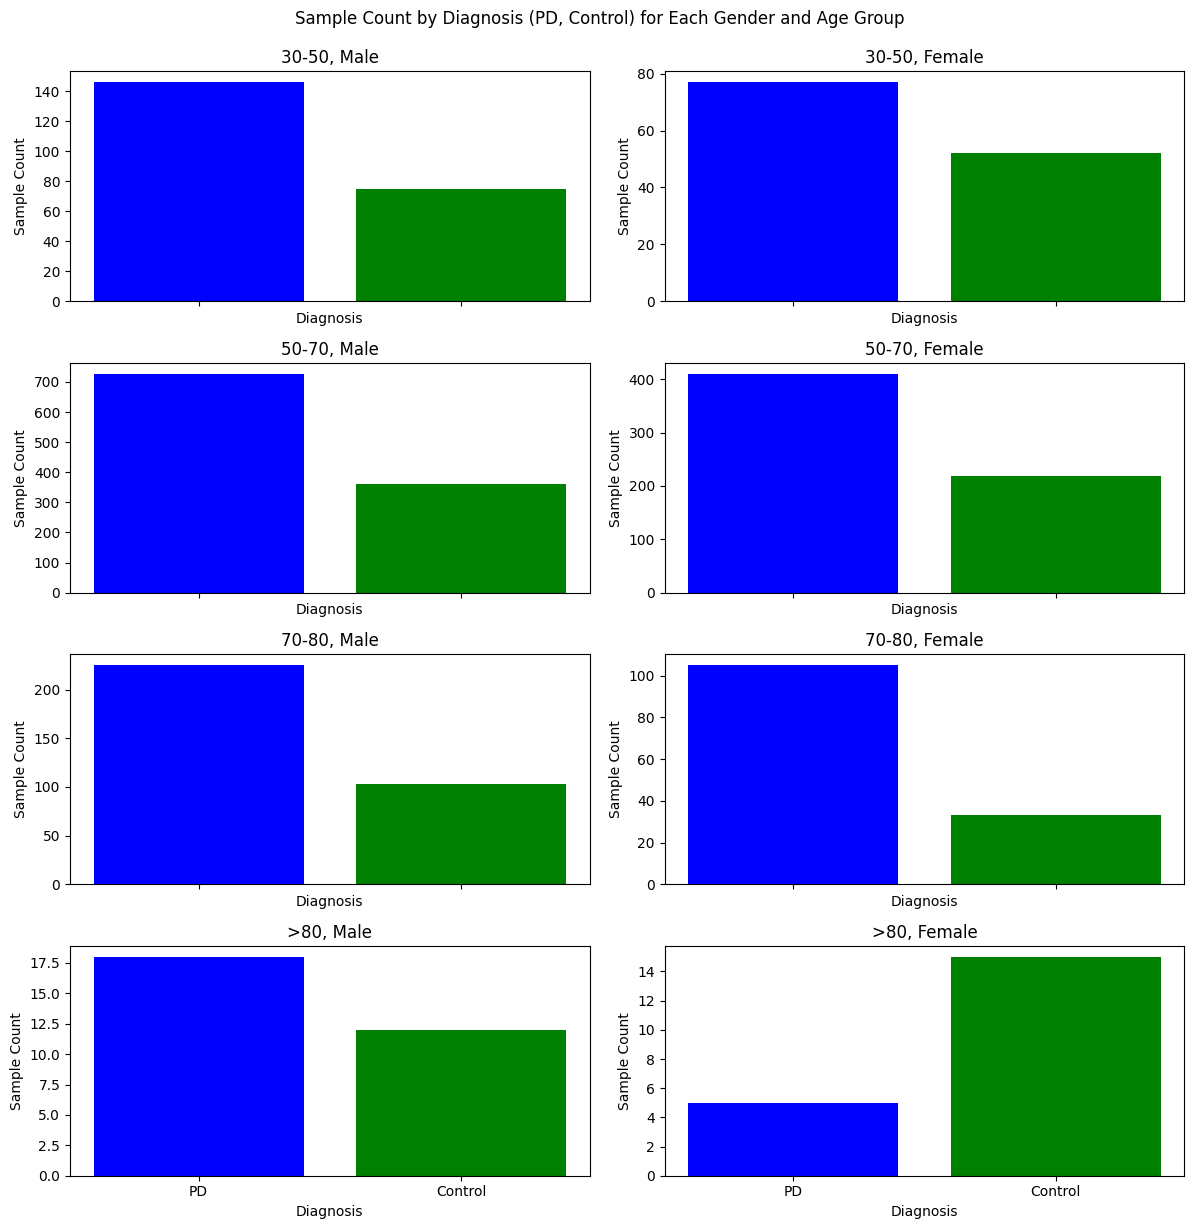
\includegraphics[width=0.7\textwidth]{ML/ppmi-visual-bar-class-imb.png}
                \caption[Απεικόνιση ανισορροπίας μεταξύ των ομάδων της μελέτης] {Στις ομάδες ανδρών 30-50, 50-70 και 70-80 παρατηρείται ανισορροπία κατά περίπου το διπλάσιο της ομάδας ελέγχου. Στις ομάδες γυναικών 50-70 επίσης, ενώ στην ηλικιακή ομάδα 70-80 περίπου το τριπλάσιο. Η ομάδα γυναικών στις ηλικίες άνω των 80 δείχνει σχεδόν τριπλάσια δείγματα ελέγχου αντί νοσούντων.}
                \label{fig:ppmi-visual-bar-class-imb}
            \end{figure}
            \par
                
    \section{Ανάλυση εμπλουτισμού}
        \par 
            Μέσω της ανάλυσης εμπλουτισμού (\emph{GSEA}) παρέχεται η διασταύρωση ενός συνόλου γονιδίων, όπως αυτά που αναδείχθηκαν ως διαφορικά εκφραζόμενα και στατιστικά σημαντικά στην προηγούμενη ενότητα, με δεδομένα σχολιασμού από βάσεις δεδομένων βιολογικών μονοπατιών, κυτταρικών λειτουργιών, φαινοτύπων κ.ά.
        \par
            Αντίστοιχα με την στρωματοποίηση, όπως αυτή πραγματοποιήθηκε στην ανάλυση διαφορικής έκφρασης γονιδίων, διεξήχθη ανάλυση εμπλουτισμού με τη χρήση των DEG\nomenclature{DEG}{Differentially Expressed Genes} ανά φύλο και ηλικιακή ομάδα. Στατιστικά σημαντικά αποτελέσματα προέκυψαν, μετά από εκτέλεση του κώδικα~\ref{lst:gseastratifiedbatchconsolidatedvisits}, για όλες τις ηλικιακές ομάδες ανά φύλο πλην ανδρών ηλικίας 50-70 ετών.
            
        \subsection{Αποτελέσματα ηλικιακής ομάδας 30-50 ετών}
            \par
            \subsubsection{Γυναίκες}
                \par
                    Στους όρους εμπλουτισμού βιολογικών διεργασιών, όπως απεικονίζονται στην εικόνα~\ref{fig:gsea_results_Female_30-50_GO_Biological_Process_2023_heatmap} παρατηρούνται κυρίως σχέσεις με μονοπάτια και αποκρίσεις του ανοσοποιητικού σε ιούς, συγκεκριμένα από τις οντολογίες GO:0045071, GO:0048525, GO:0045069 όπου αποδίδεται το υψηλότερο σκορ σύμφωνα με τις τιμές $padj$.
                \begin{figure}[H]
                    \centering
                    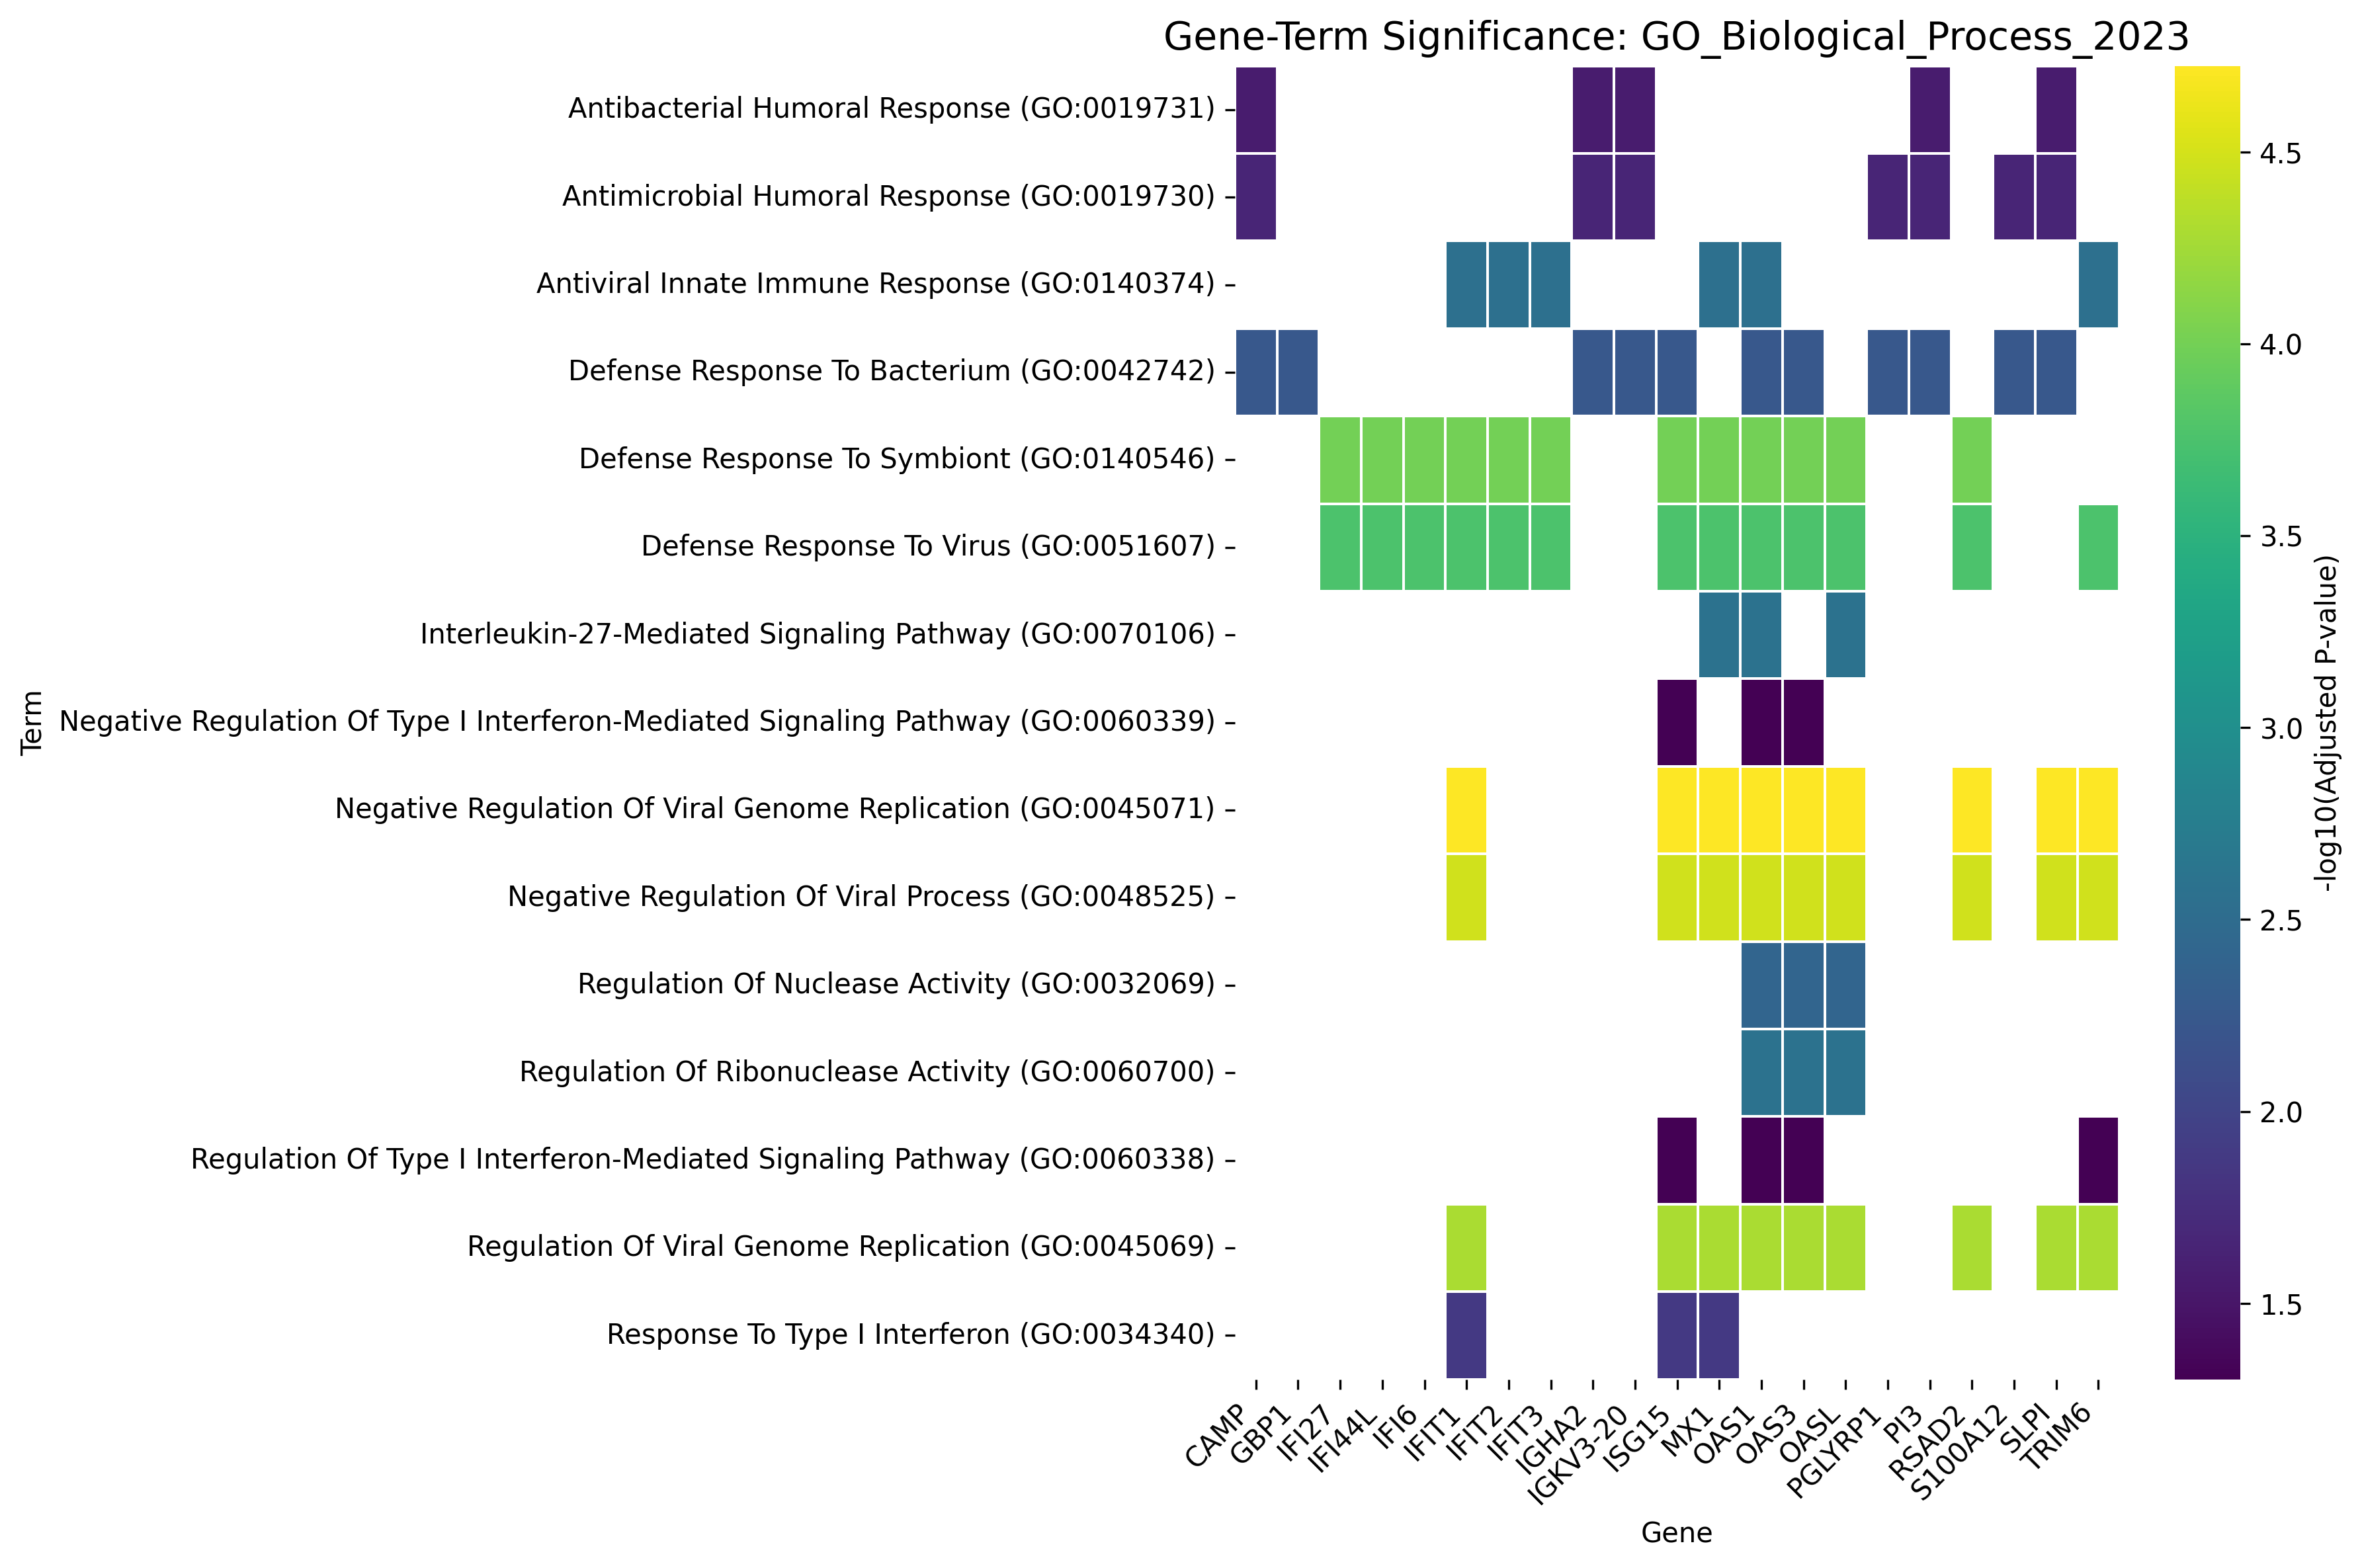
\includegraphics[width=0.8\textwidth]{GSEA/Females/30-50/gsea_results_Female_30-50_GO_Biological_Process_2023_heatmap.png}
                    \caption{Αποτελέσματα GSEA γυναικών ηλικίας 30-50 ετών}
                    \label{fig:gsea_results_Female_30-50_GO_Biological_Process_2023_heatmap}
                \end{figure}
            \subsubsection{Ανδρες}
                \par
                    Οι όροι εμπλουτισμού που επιστράφηκαν από την ανάλυση εμπλουτισμού είναι μερικώς όμοιοι με αυτούς των γυναικών καθώς και γενικότερα τα αποτελέσματα για τους άνδρες σχετίζονται επίσης με τη βιολογία του ανοσοποιητικού.
                \begin{figure}[H]
                    \centering
                    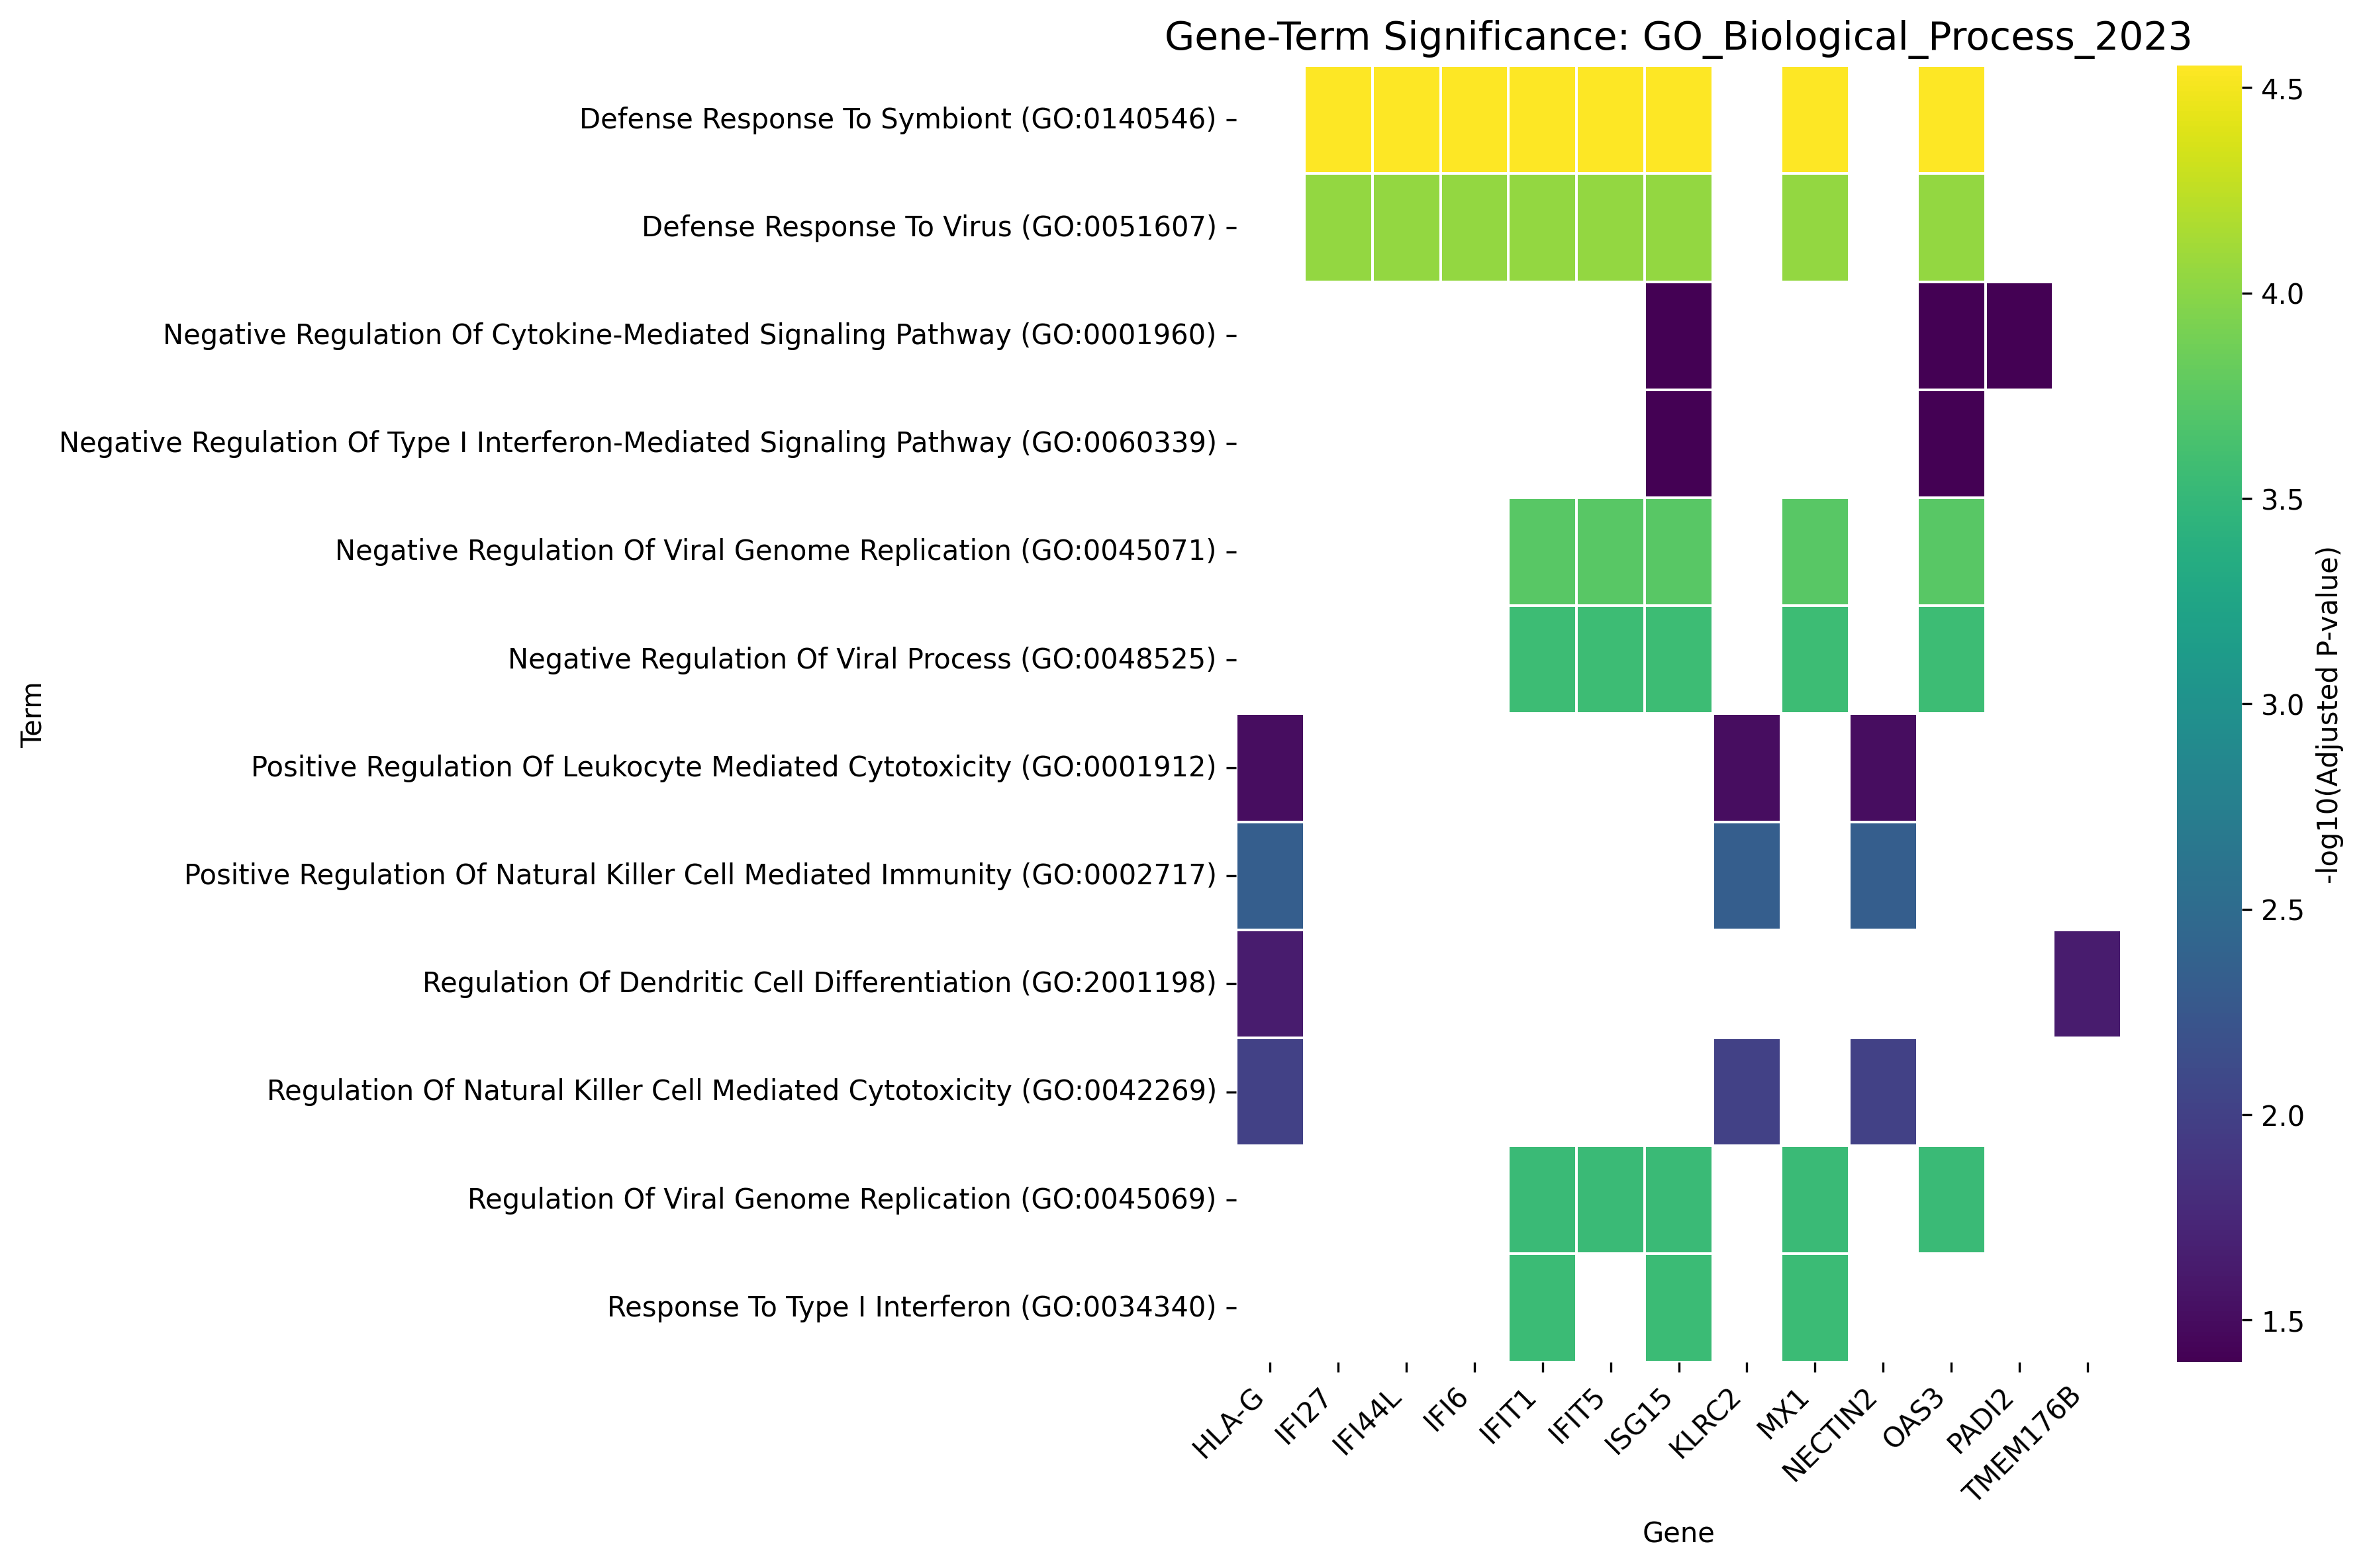
\includegraphics[width=0.8\textwidth]{GSEA/Males/30-50/gsea_results_Male_30-50_GO_Biological_Process_2023_heatmap.png}
                    \caption{Αποτελέσματα GSEA ανδρών ηλικίας 30-50 ετών}
                    \label{fig:gsea_results_Male_30-50_GO_Biological_Process_2023_heatmap}
                \end{figure}
            \newpage
        \subsection{Αποτελέσματα ηλικιακής ομάδας 50-70 ετών}
            \subsubsection{Γυνάικες}
            \par
                Τα αποτελέσματα της ηλικιακής ομάδας 50-70 ετών στις γυναίκες δείχνουν παρόμοια αποτελέσματα όπως και της ομάδας 30-50 ετών. Οι σχολιασμοί σχετίζονται και εδώ με βιολογικές διεργασίες του ανοσοποιητικού σχετικά με ιογενή μόλυνση.
            \begin{figure}[H]
                \centering
                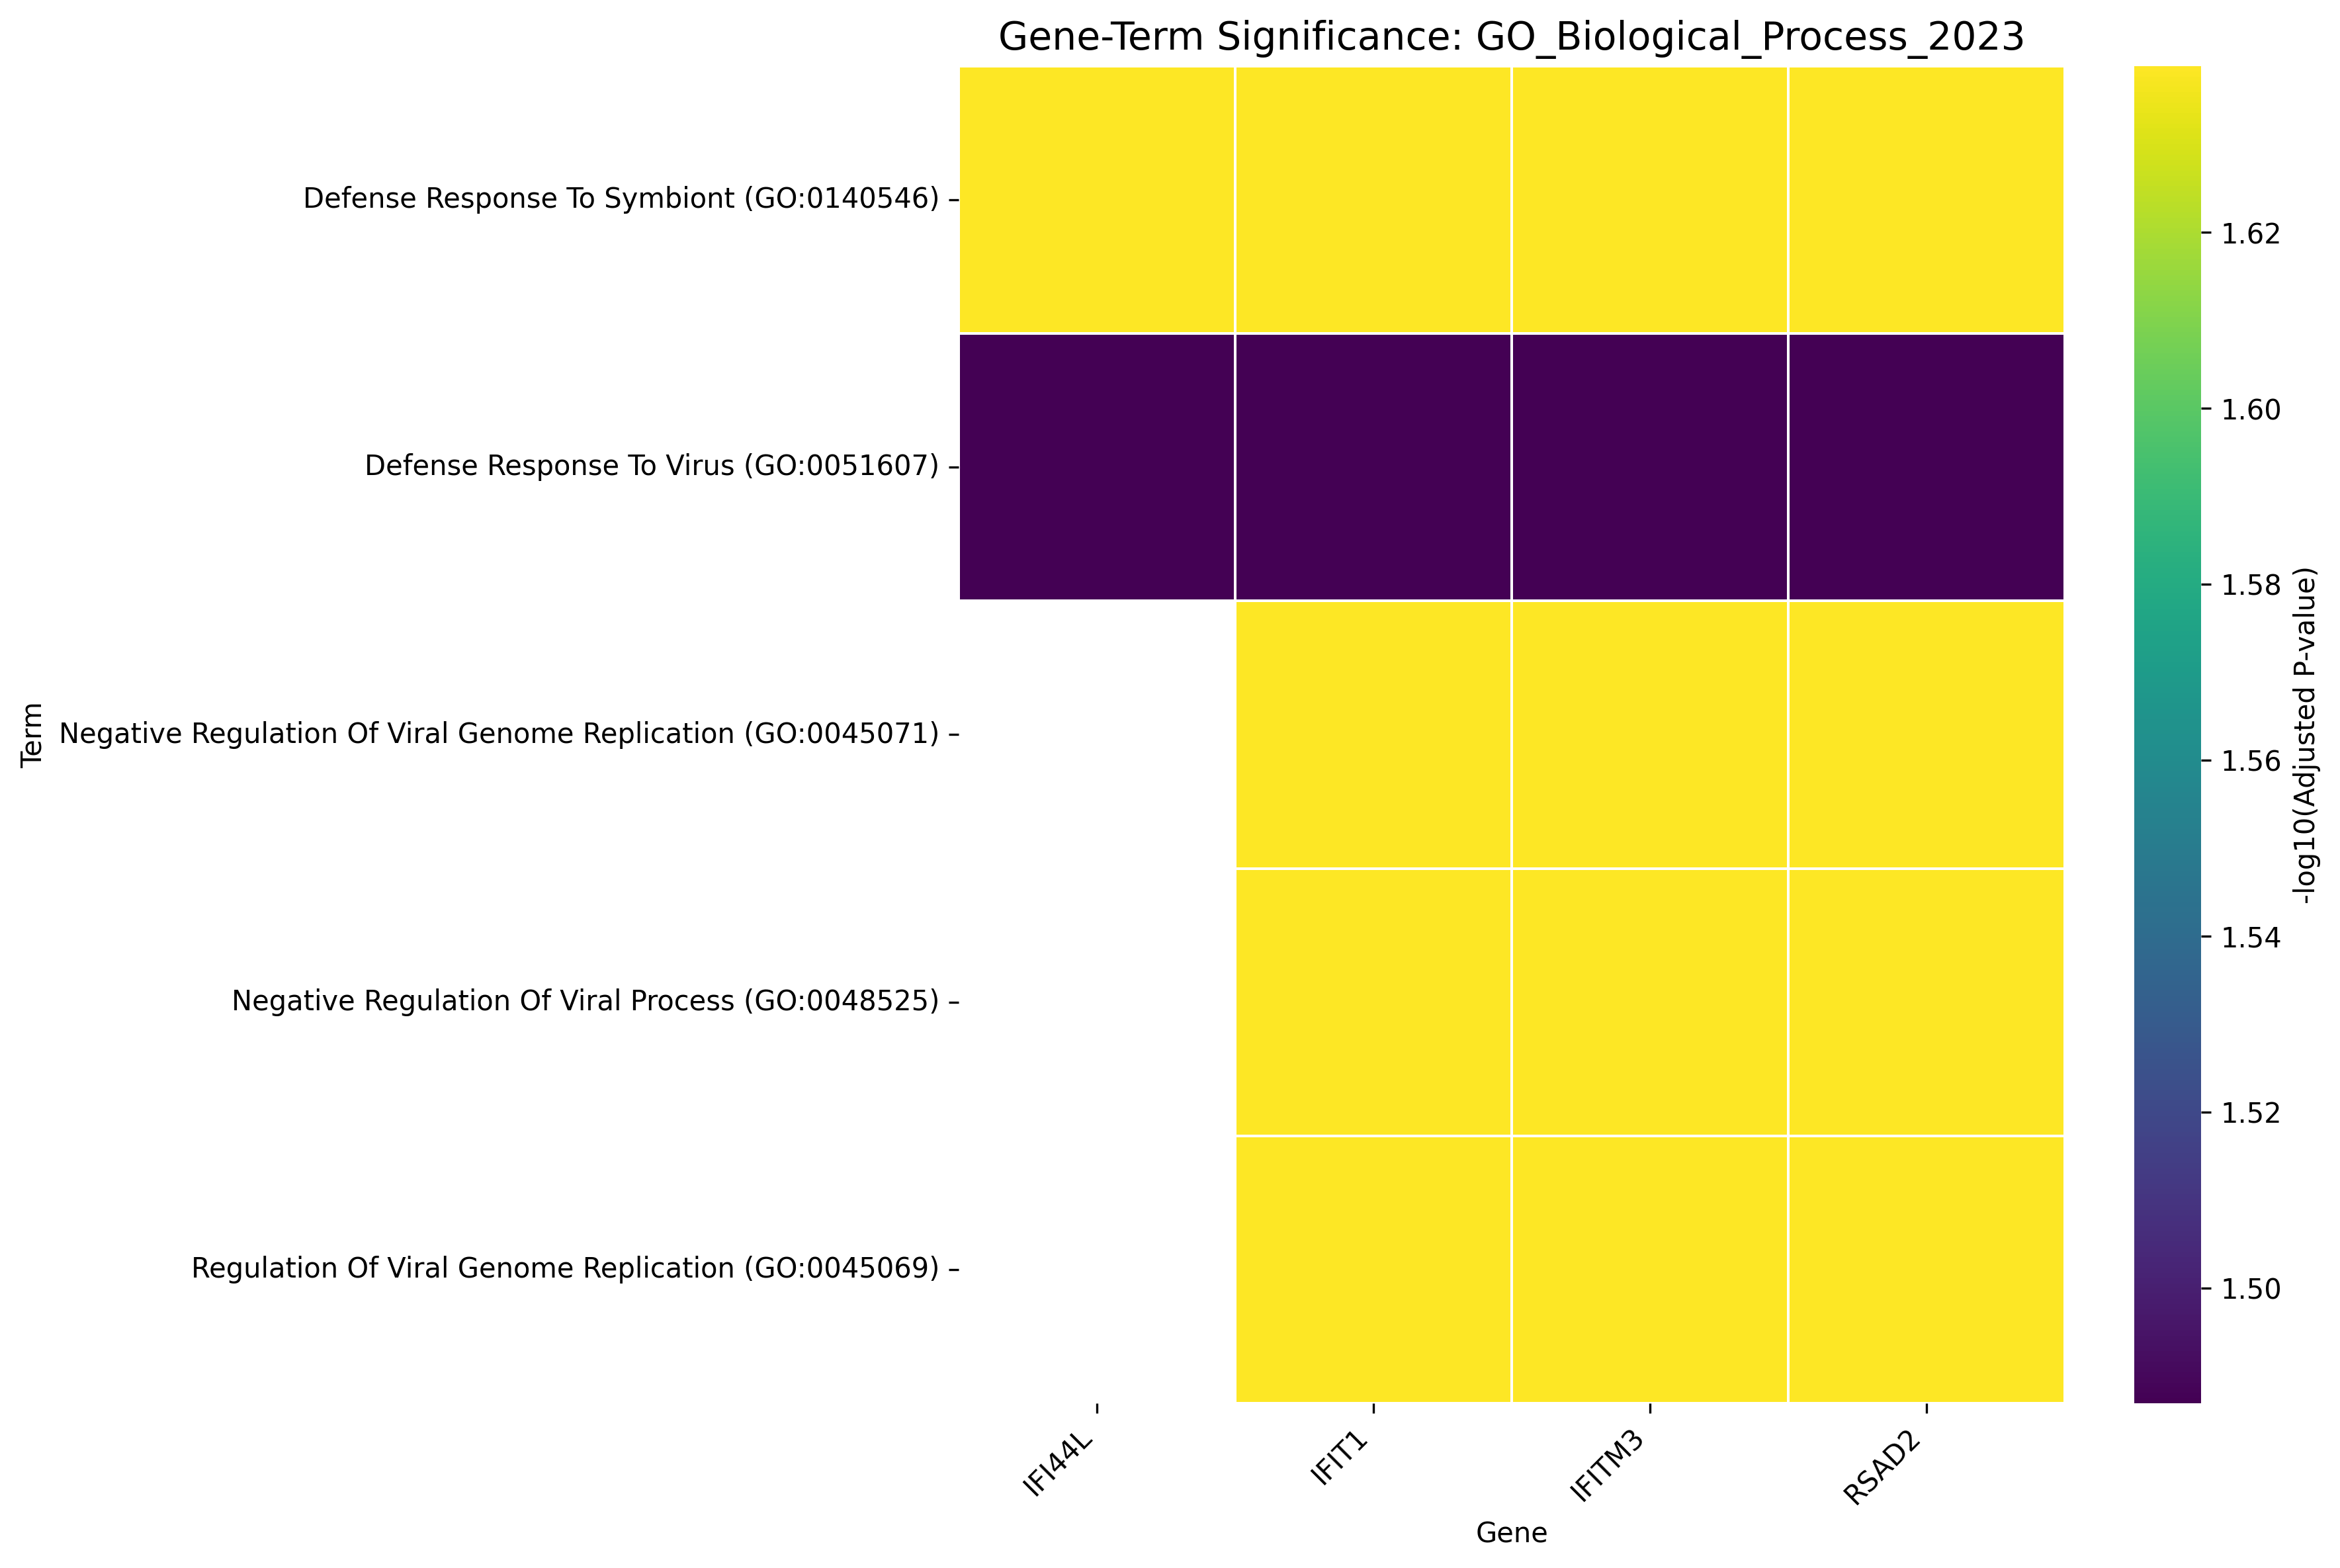
\includegraphics[width=0.8\textwidth]{GSEA/Females/50-70/gsea_results_Female_50-70_GO_Biological_Process_2023_heatmap.png}
                \caption{Αποτελέσματα GSEA γυναικών ηλικίας 50-70 ετών}
                \label{fig:gsea_results_Female_50-70_GO_Biological_Process_2023_heatmap}
            \end{figure}
        

    % \subsection{First Subsection}
    % \subsubsection{First Subsubsection}

    % Add abbreviations where they're first used
    % \nomenclature{AU}{Astronomical Unit}
    % \nomenclature{CPU}{Central Processing Unit}
    
    % Text with 12pt font, justified alignment, and 1.5 line spacing.
    
    % \begin{figure}[H]
    %     \centering
    %     \includegraphics[width=0.5\textwidth]{example-image}
    %     \caption{Example figure caption}
    % \end{figure}
    
    % \begin{table}[H]
    %     \centering
    %     \begin{tabular}{ll}
    %         Header 1 & Header 2 \\
    %         Content 1 & Content 2 \\
    %     \end{tabular}
    %     \caption{Example table caption}
    % \end{table}

    \cleardoublepage
    \appendix
    \chapter*{Παράρτημα}
    \addcontentsline{toc}{chapter}{Παράρτημα}
    
    \section*{Κώδικας Προγραμμάτων}\label{thesis:code}
    % \lstset{language=R}
    \begin{lstlisting}[language=Python,caption={read-data.py: Συκγρότηση CSV αρχείου με το σύνολο των δειγμάτων},label=lst:readdatapy]
    import pandas as pd
    import numpy as np
    import glob
    import os
    from tqdm import tqdm
    from multiprocessing import Pool, cpu_count
    
    def read_csv(filename):
        df = pd.read_csv(filename, sep="\t", comment="#", header=None, skiprows=1)
        df.columns = ["GeneID", "Chr", "Start", "End", "Strand", "Length", "Counts"]
        df = df[["GeneID", "Counts"]].set_index("GeneID")
        df.rename(columns={"Counts": os.path.basename(filename)}, inplace=True)
        return df
    
    def main():
        num_workers = min(6, cpu_count())
        count_files = glob.glob("/Volumes/Elements/counts/*.txt")
        count_files_len = len(count_files)
        count_files_len=10
        all_counts = []
        with Pool(num_workers) as pool:
            for result in tqdm(pool.imap_unordered(read_csv, count_files[1:10]), total=count_files_len, desc="Reading files"):
                all_counts.append(result)
    
        all_counts = pd.concat(all_counts, axis=1, join="outer")
        all_counts = all_counts.apply(pd.to_numeric, errors="coerce").fillna(0)
        all_counts.to_csv("ppmi_counts_matrix.csv", index=True)
    
        print("Done")

        if __name__ == '__main__':
            main()
    \end{lstlisting}
    \begin{lstlisting}[language=Python,caption={prepare-data.py: Εισαγωγή Metadata και φιλτράρισμα ακατάλληλων δειγμάτων},label=lst:preparedatapy]
        import pandas as pd
    
        def main():
            metadata = pd.read_csv("/Volumes/Elements/metaDataIR3.csv")
            metadata = metadata[metadata["QCflagIR3"].str.lower() == "pass"]
            counts = pd.read_csv("ppmi_counts_matrix.csv")
        
            counts = counts.set_index("GeneID")
            pattern = r"(\d+\-SL-\d+)"
            new_colnames = counts.columns.str.extract(pattern, expand=False)
            counts.columns = new_colnames
            metadata = metadata.set_index("HudAlphaID")
            merged = metadata.join(counts.T)
            merged.to_csv("ppmi_clean_counts_meta.csv")
        
        if __name__ == '__main__':
            main()
    \end{lstlisting}
    \begin{lstlisting}[language=Python,caption={data\_consolidation.py: Συγχώνευση δεδομένων σε H5AD τύπο αρχείου}, label=lst:dataconsolidationpy]
        import pandas as pd
        import mygene
        import re
        import anndata as ad
        import numpy as np
        import anndata as ad
        import numpy as np
        
        genetic_mapping = {
            'ENRLPINK1': 'PINK1',
            'ENRLPRKN': 'PRKN',
            'ENRLSRDC': 'SRDC',
            'ENRLHPSM': 'HPSM',
            'ENRLRBD': 'RBD',
            'ENRLLRRK2': 'LRRK2',
            'ENRLSNCA': 'SNCA',
            'ENRLGBA': 'GBA'
        }
        
        def get_genetic_group(row):
            for col, group in genetic_mapping.items():
                if row[col] == 1:
                    return group
            return 'None'
        
        def map_age_group(age):
            if 30 <= age <= 50:
                return "30-50"
            elif 50 < age <= 70:
                return "50-70"
            elif 70 < age <= 80:
                return "70-80"
            elif age > 80:
                return ">80"
            return "Unknown"
        
        def main():
            bulk_feature_counts = pd.read_csv("/Users/kpax/Documents/aep/study/MSC/lab/PPMI_Project_133_RNASeq/ppmi_counts_meta_dataset.csv", index_col=0)
            patient_status = pd.read_csv("/Users/kpax/Documents/aep/study/MSC/lab/PPMI_Project_133_RNASeq/Participant_Status_19Mar2025.csv")
            genetic_groups = patient_status[['PATNO'] + list(genetic_mapping.keys())].copy()
            genetic_groups['Genetic_Group'] = genetic_groups.apply(get_genetic_group, axis=1)
            bulk_feature_counts = bulk_feature_counts.merge(
                genetic_groups[['PATNO', 'Genetic_Group']],
                left_on='Patient',
                right_on='PATNO',
                how='left'
            ).set_index(bulk_feature_counts.index)
        
            counts_raw = bulk_feature_counts.iloc[:,bulk_feature_counts.columns.str.startswith("ENSG")]
            counts_raw_t = counts_raw.T
            trunc_eid = [re.sub(r"\.\d+$", "", eid) for eid in counts_raw_t.index.values.tolist()]
        
            mg = mygene.MyGeneInfo()
            mappings = mg.querymany(
                trunc_eid,
                scopes="ensembl.gene",
                fields="symbol",
                species="human"
            )
            df = pd.DataFrame(mappings)
            df = df[['query', 'symbol']].rename(columns={'query': 'Ensembl_ID', 'symbol': 'Gene_Symbol'})
            df['Gene_Symbol'] = df['Gene_Symbol'].fillna(df['Ensembl_ID'])
            dup_counts = df['Ensembl_ID'].value_counts()
            print(f"Total duplicates: {len(dup_counts[dup_counts > 1])}")
            print(dup_counts[dup_counts > 1])
        
        
            df_deduped = df.drop_duplicates(subset=['Ensembl_ID'], keep='first')
            counts_raw_export = counts_raw_t.reset_index(drop=False)
            counts_raw_export['index'] = trunc_eid
            counts_raw_export = counts_raw_export.rename(columns={'index':'Ensembl_ID'})
            counts_raw_export = (
                counts_raw_export.merge(df_deduped, on='Ensembl_ID', how='left')
                .set_index('Gene_Symbol')
                .drop(columns=['Ensembl_ID'])
            )
        
            bulk_feature_counts['Genetic_Group'] = bulk_feature_counts['Genetic_Group'].fillna('Unknown')
        
            patient_status['Age_Group'] = patient_status['ENROLL_AGE'].apply(map_age_group)
        
            age_group_mapping = patient_status[['PATNO', 'Age_Group']]
        
            bulk_feature_counts = bulk_feature_counts.merge(
                age_group_mapping,
                left_on='Patient',
                right_on='PATNO',
                how='left'
            ).set_index(bulk_feature_counts.index)
        
            counts_raw_export.index.name = None
        
            ensembl_symbol_mapping = pd.DataFrame({
                "gene_symbol": counts_raw_export.index,
                "ensembl_id": counts_raw_t.index,
                "trunc_eid": trunc_eid
            }).set_index('ensembl_id')
        
            ppmi_adata = ad.AnnData(bulk_feature_counts.loc[:, bulk_feature_counts.columns.str.startswith("ENSG")])
            ppmi_adata.obs['Sample'] = bulk_feature_counts['Sample'].values
            ppmi_adata.obs['Diagnosis'] = bulk_feature_counts['Diagnosis'].values
            ppmi_adata.obs['Visit'] = bulk_feature_counts['Visit'].values
            ppmi_adata.obs['Gender'] = bulk_feature_counts['Gender'].values
            ppmi_adata.obs['Patient'] = bulk_feature_counts['Patient'].values
            ppmi_adata.obs['Genetic_Group'] = bulk_feature_counts['Genetic_Group'].values
            ppmi_adata.obs['Age_Group'] = bulk_feature_counts['Age_Group'].values
            ppmi_adata.layers['counts_log2'] = np.log2(ppmi_adata.X + 1)
            ppmi_adata.layers['gene_symbols'] = counts_raw_export.T
            ppmi_adata.varm['symbol_ensembl_mapping'] = ensembl_symbol_mapping
        
            ppmi_adata.write_h5ad("/Users/kpax/Documents/aep/study/MSC/lab/PPMI_Project_133_RNASeq/ppmi_adata.h5ad")
        
        if __name__ == '__main__':
            main()
    \end{lstlisting}
    \begin{lstlisting}[language=R,caption={Main.R: Διαφορική ανάλυση μέσω πακέτου R DESeq2},label=lst:mainr]
        library(DESeq2)
        library(tibble)
        library(tidyverse)
        
        setwd('/Users/kpax/Documents/aep/study/MSC/lab/PPMI_Project_133_RNASeq')
        
        metadata <- read.csv("metadata.csv", row.names=1)
        counts <-  read.csv("counts_matrix.csv", row.names=1)
        
        design <- "Visit + Diagnosis"
        
        strata <- list(
          list(Gender="Male", Age_Group="30-50", Diagnosis=c("PD", "Control"), Design=design),
          list(Gender="Male", Age_Group="50-70", Diagnosis=c("PD", "Control"), Design=design),
          list(Gender="Male", Age_Group="70-80", Diagnosis=c("PD", "Control"), Design=design),
          list(Gender="Male", Age_Group=">80", Diagnosis=c("PD", "Control"), Design=design),
          list(Gender="Female", Age_Group="30-50", Diagnosis=c("PD", "Control"), Design=design),
          list(Gender="Female", Age_Group="50-70", Diagnosis=c("PD", "Control"), Design=design),
          list(Gender="Female", Age_Group="70-80", Diagnosis=c("PD", "Control"), Design=design),
          list(Gender="Female", Age_Group=">80", Diagnosis=c("PD", "Control"), Design=design)
        )
        
        results_list <- lapply(strata, function(stratum) {
          print(paste("design=",stratum$Design))
          meta_stratum <- metadata %>% filter(Gender == stratum$Gender,
                                              Age_Group == stratum$Age_Group,
                                              # Visit == stratum$Visit,
                                              Diagnosis %in% stratum$Diagnosis)
          counts_stratum <- counts[rownames(meta_stratum), ]
          dds <- DESeqDataSetFromMatrix(
            t(counts_stratum),
            meta_stratum,
            design = formula(paste("~ ", stratum$Design))
          )
          dds <- DESeq(dds)
          (dds)
        })
        
        
        names(results_list) <- sapply(strata, function(s) paste(s$Gender, s$Age_Group, sep="_"))
        for (i in seq_along(results_list)) {
          stratum_name <- ifelse(is.null(names(results_list)),
                                 paste0("Stratum_", i),
                                 names(results_list)[i])
          res <- results(results_list[[i]], contrast=c("Diagnosis", "PD", "Control")) %>%
            as.data.frame() %>%
            rownames_to_column("Gene") %>%
            arrange(padj, desc(abs(log2FoldChange)))
          filename <- file.path("./data/deg_consolidated_visits", paste0("DEGs_stratified_consoVisits_", stratum_name, ".csv"))
          write.csv(res, file=filename, row.names=FALSE)
        }
    \end{lstlisting}
    \begin{lstlisting}[language=Python,caption={process\_deg\_consolidated\_visits.py: Κατασκευή γραφημάτων διαφορικά εκφραζομένων γονιδίων}, label=lst:processdegconsolidatedvisitspy]
        import pandas as pd
        import matplotlib.pyplot as plt
        import numpy as np
        
        def visualize_amounts_of_up_and_down_regulated_genes(dfs):
            fig, axes = plt.subplots(1, 4, figsize=(20, 5))
            titles = list(dfs.keys())
        
            for ax, df, title in zip(axes, list(dfs.values()), titles):
                count_up = ((df['log2FoldChange'] > 0.5) & (df['padj'] < 0.05)).sum()
                count_down = ((df['log2FoldChange'] < -0.5) & (df['padj'] < 0.05)).sum()
                ax.bar(['Upregulated > 0.5', 'Downregulated < -0.5'], [count_up, count_down], color=['red', 'blue'])
                ax.set_title(title)
                ax.set_ylabel('Gene Count')
                ax.set_xlabel('Expression')
        
            plt.tight_layout()
            return plt
        
        def visualize_volcano_plots(dfs):
            fig, axes = plt.subplots(1, 4, figsize=(25, 5), sharey=False)
            titles = list(dfs.keys())
        
            for ax, df, title in zip(axes, list(dfs.values()), titles):
                significant = (df['log2FoldChange'].abs() > 0.5) & (df['padj'] < 0.05)
                ax.scatter(df['log2FoldChange'], -np.log10(df['padj']), color='gray', s=10, alpha=0.6, label='Non-significant')
                ax.scatter(df.loc[significant, 'log2FoldChange'],
                           -np.log10(df.loc[significant, 'padj']),
                           color='red',
                           s=10,
                           label='Significant')
                ax.axvline(x=0.5, color='blue', linestyle='--', linewidth=0.8)
                ax.axvline(x=-0.5, color='blue', linestyle='--', linewidth=0.8)
                ax.set_title(title)
                ax.set_xlabel('log$_2$ Fold Change')
                ax.set_ylabel('-log$_{10}$(p-value)')
                ax.legend(loc='upper right', fontsize='small')
        
            plt.tight_layout()
            return plt
        
        def main():
            gender = ["Male", "Female"]
            age_groups = ["30-50", "50-70", "70-80", ">80"]
        
            deg_data_path = "/Users/kpax/Documents/aep/study/MSC/lab/PPMI_Project_133_RNASeq/data/deg_consolidated_visits/"
            deg_results_path = "/Users/kpax/Documents/aep/study/MSC/lab/PPMI_Project_133_RNASeq/data/deg_consolidated_visits/results"
        
            dfs = {};
            dfs_filtered = {};
            for gender in gender:
                for age_group in age_groups:
                    df = pd.read_csv(deg_data_path + f"DEGs_stratified_consoVisits_{gender}_{age_group}.csv")
                    df_filtered = df[(df['log2FoldChange'].abs() > 0.5) & (df['padj'] < 0.05)]
                    dfs_filtered[age_group] = df_filtered
                    dfs[age_group] = df
        
                volcano_plot = visualize_volcano_plots(dfs)
                volcano_plot.savefig(deg_results_path + f"/volcano_plot_consoVisits_{gender}.png")
                bar_plot = visualize_amounts_of_up_and_down_regulated_genes(dfs)
                bar_plot.savefig(deg_results_path + f"/barplot_plot_consoVisits_{gender}.png")
        
        
        if __name__ == '__main__':
            main()
        
    \end{lstlisting}
    \begin{lstlisting}[language=Python,caption={gsea\_stratified\_batch\_consolidated\_visits.py: Ανάλυση εμπλουτισμού με χρήση της βιβλιοθήκης gseapy σε Python}, label=lst:gseastratifiedbatchconsolidatedvisits]
    from typing import Final
        import anndata as ad
        import pandas as pd
        import numpy as np
        import gseapy as gp
        
        DEG_DATA_PATH: Final = "/Users/kpax/Documents/aep/study/MSC/lab/PPMI_Project_133_RNASeq/data/deg_consolidated_visits"
        GSEA_PATH: Final = "/Users/kpax/Documents/aep/study/MSC/lab/PPMI_Project_133_RNASeq/data/gsea"
        
        
        def main():
            ppmi_ad = ad.read_h5ad("/Users/kpax/Documents/aep/study/MSC/lab/PPMI_Project_133_RNASeq/ppmi_adata.h5ad")
            age_groups = ['30-50', '50-70', '70-80', '>80']
            genders = ['Male', 'Female']
            gene_sets = ['MSigDB_Hallmark_2020',
                         'KEGG_2021_Human',
                         'WikiPathways_2024_Human',
                         'Human_Phenotype_Ontology',
                         'GO_Biological_Process_2023',
                         'GO_Molecular_Function_2023',
                         'GO_Cellular_Component_2023',
                         'SynGO_2024',
                         'OMIM_Disease',
                         'ARCHS4_TFs_Coexp',
                         'ChEA_2013',
                         'ChEA_2015',
                         'ChEA_2016',
                         'ChEA_2022',
                         'ENCODE_TF_ChIP-seq_2014',
                         'ENCODE_TF_ChIP-seq_2015',
                         'ENCODE_and_ChEA_Consensus_TFs_from_ChIP-X',
                         'Enrichr_Submissions_TF-Gene_Coocurrence',
                         'TF-LOF_Expression_from_GEO',
                         'TF_Perturbations_Followed_by_Expression',
                         'TRRUST_Transcription_Factors_2019']
        
            for gender in genders:
                for age_group in age_groups:
                    print(f"GSEA running => Age Group: {age_group}, Gender: {gender}")
                    mask = ((ppmi_ad.obs['Age_Group'] == age_group) &
                            (ppmi_ad.obs['Gender'] == gender) &
                            (ppmi_ad.obs['Diagnosis'].isin(['PD', 'Control'])))
        
                    ppmi_ad_subset = ppmi_ad[mask]
                    symbol_ensembl_mapping = ppmi_ad_subset.varm['symbol_ensembl_mapping']
                    deg_data = pd.read_csv(f"{DEG_DATA_PATH}/DEGs_stratified_consoVisits_{gender}_{age_group}.csv", index_col=0)
                    deg_sign = deg_data[
                        (np.abs(deg_data['log2FoldChange']) > 0.5) & (deg_data['padj'] < 0.05)]
                    deg_sign = deg_sign.merge(symbol_ensembl_mapping, left_index=True, right_index=True)
                    ranked_genes = deg_sign.set_index('gene_symbol')['stat'].sort_values(ascending=False)
                    ranked_genes = ranked_genes[~ranked_genes.isna()]
                    ranked_genes = ranked_genes.sort_values(ascending=False, key=abs)
                    if ranked_genes.empty:
                        continue
        
                    enr = gp.enrichr(gene_list=ranked_genes.index.tolist(),
                                     gene_sets=gene_sets,
                                     organism='human',
                                     verbose=True)
                    enr_results_sorted = enr.results.sort_values(by='Adjusted P-value', ascending=True)
                    enr_results_sorted.to_csv(f"{GSEA_PATH}/enr_results_sorted_consoVisits_{gender}_{age_group}.csv")
        
        
        if __name__ == '__main__':
            main()
    \end{lstlisting}
    
    % \section*{Επιπλέον Υλικά}
    % [Your additional appendix content...]

    \printbibliography

\end{document}